%%%%%%%%%%%%%%%%%%%%%%%%%%%%%%%%%%%%%%%%%%%%%%%%%%%%%%
\hide{ % hide the old results section
In this work, we examine the effectiveness of \ts with middle grade students. Our analysis focused on the students' performance and completeness on the worksheets as well as the scores of their Modify and Create Projects. We explored the effects of various internal (student-based), external (environment-based), and question-specific factors on student interaction with the worksheets, and how their \ts{} scores correlated with their project scores. This resulted in four sets of results. We then synthesize our findings with respect to each other and our research questions in Section \ref{sec:discussion}.

\newcounter{findingnum}

\subsection{Environment-based Factors}

%We begin our presentation of findings with overall results highlighting the effectiveness of \ts as a learning strategy for middle grade students, before then exploring particular behaviors noticed in students engaging with the strategy. The overall results are broken into two subfindings: the effects of student-based factors (i.e. parent-reported previous relevant academic and extra-curricular experience) and environment-based factors (i.e. learning environment and curriculum structure).
First, we discuss the environmental factors. These factors include the students' grade levels, teachers, and the modules of the curriculum.

\stepcounter{findingnum}
\textit{Finding \arabic{findingnum}: Students using \ts{} performed similarly well in all grade levels across two \scratchencore{} modules but overall, they differed in performance based on module and teacher.} 

Figure \ref{fig:classroom_factors} illustrates the difference in \ts{} worksheet performance by grade level and teacher. The average \ts{} composite score for grade 4 students was 91.24\%, 90.84\% for grade 5, 94.53\% for grade 6, and 90.90\% for grade 7. For Module 2 - Events and Module 4 - Conditional Loops, students across all grade levels completed the worksheets with similar correctness (\begin{math}M2: F(2,209)=.0158, p=.984; M4:\chi=3.391, p=.0656\end{math}). In contrast, for Module 1 - Scratch Basics and Module 3 - Animation, grade level was linked to worksheet correctness (\begin{math}M1: F(3, 255)=4.30, p<.01, \eta^2=.0482; M3:\chi=23.79, p<.01, \eta^2=.0747\end{math}). Post-hoc comparisons for Module 1 - Scratch Basics reveal significant differences in correctness between 6th graders and both 4th and 7th graders (\begin{math}p<.05\end{math}). For Module 3 - Animation, 7th graders performed better than 5th graders (\begin{math}p<.01\end{math}). It is interesting to note that while there was a difference between Module 1 - Scratch Basics and Module 3 - Animation, there were no differences between 5th and 6th graders for Module 4 - Conditional Loops.

Next, we examined the results when stratified by the particular modules within the curriculum, allowing us to observe whether certain elements of the curriculum itself (considered to be an environmental factor) affected student success. The results of this stratification by content are provided in Figure \ref{fig:curriculum_factors}. The average composite score for Module 1 - Scratch Basics was 91.12\%, 91.97\% for Module 2 - Events, 88.78\% for Module 3 - Animation, and 91.88\% for Module 4 - Conditional Loops. Our statistical analysis revealed that student worksheet correctness was different across the different modules (\begin{math}F(3,668)=4.10, p<0.01, \eta^2=.0181\end{math}).

Finally, we investigated whether there was a difference in student performance on the worksheets based on the teachers (Figure \ref{fig:teacher_factors}). Average composite scores by teacher ranged from 88.75\% to 93.64\%, with a median of 91.62\% and a standard deviation of 1.86\%. For all modules, the teacher was significantly linked to worksheet correctness (\begin{math}M1: \chi=40.52, p<.01, \eta^2=.112; M2: \chi=13.10, p<.05, \eta^2=.0235, M3: \chi=29.85, p<.05, \eta^2=.0886, M4: \chi=9.50, p<.01, \eta^2=.0247\end{math}). This result echos previous findings on student performance using \ts \cite{franklin2020analysis}.

\begin{figure}
    \centering
    \includegraphics[width=.5\textwidth]{Modules.png}
    \caption{\ts Scores Compared Across Modules}
    \label{fig:curriculum_factors}
\end{figure}

\begin{figure}
     \centering
    \begin{subfigure}[t]{0.49\textwidth}
        \raisebox{-\height}{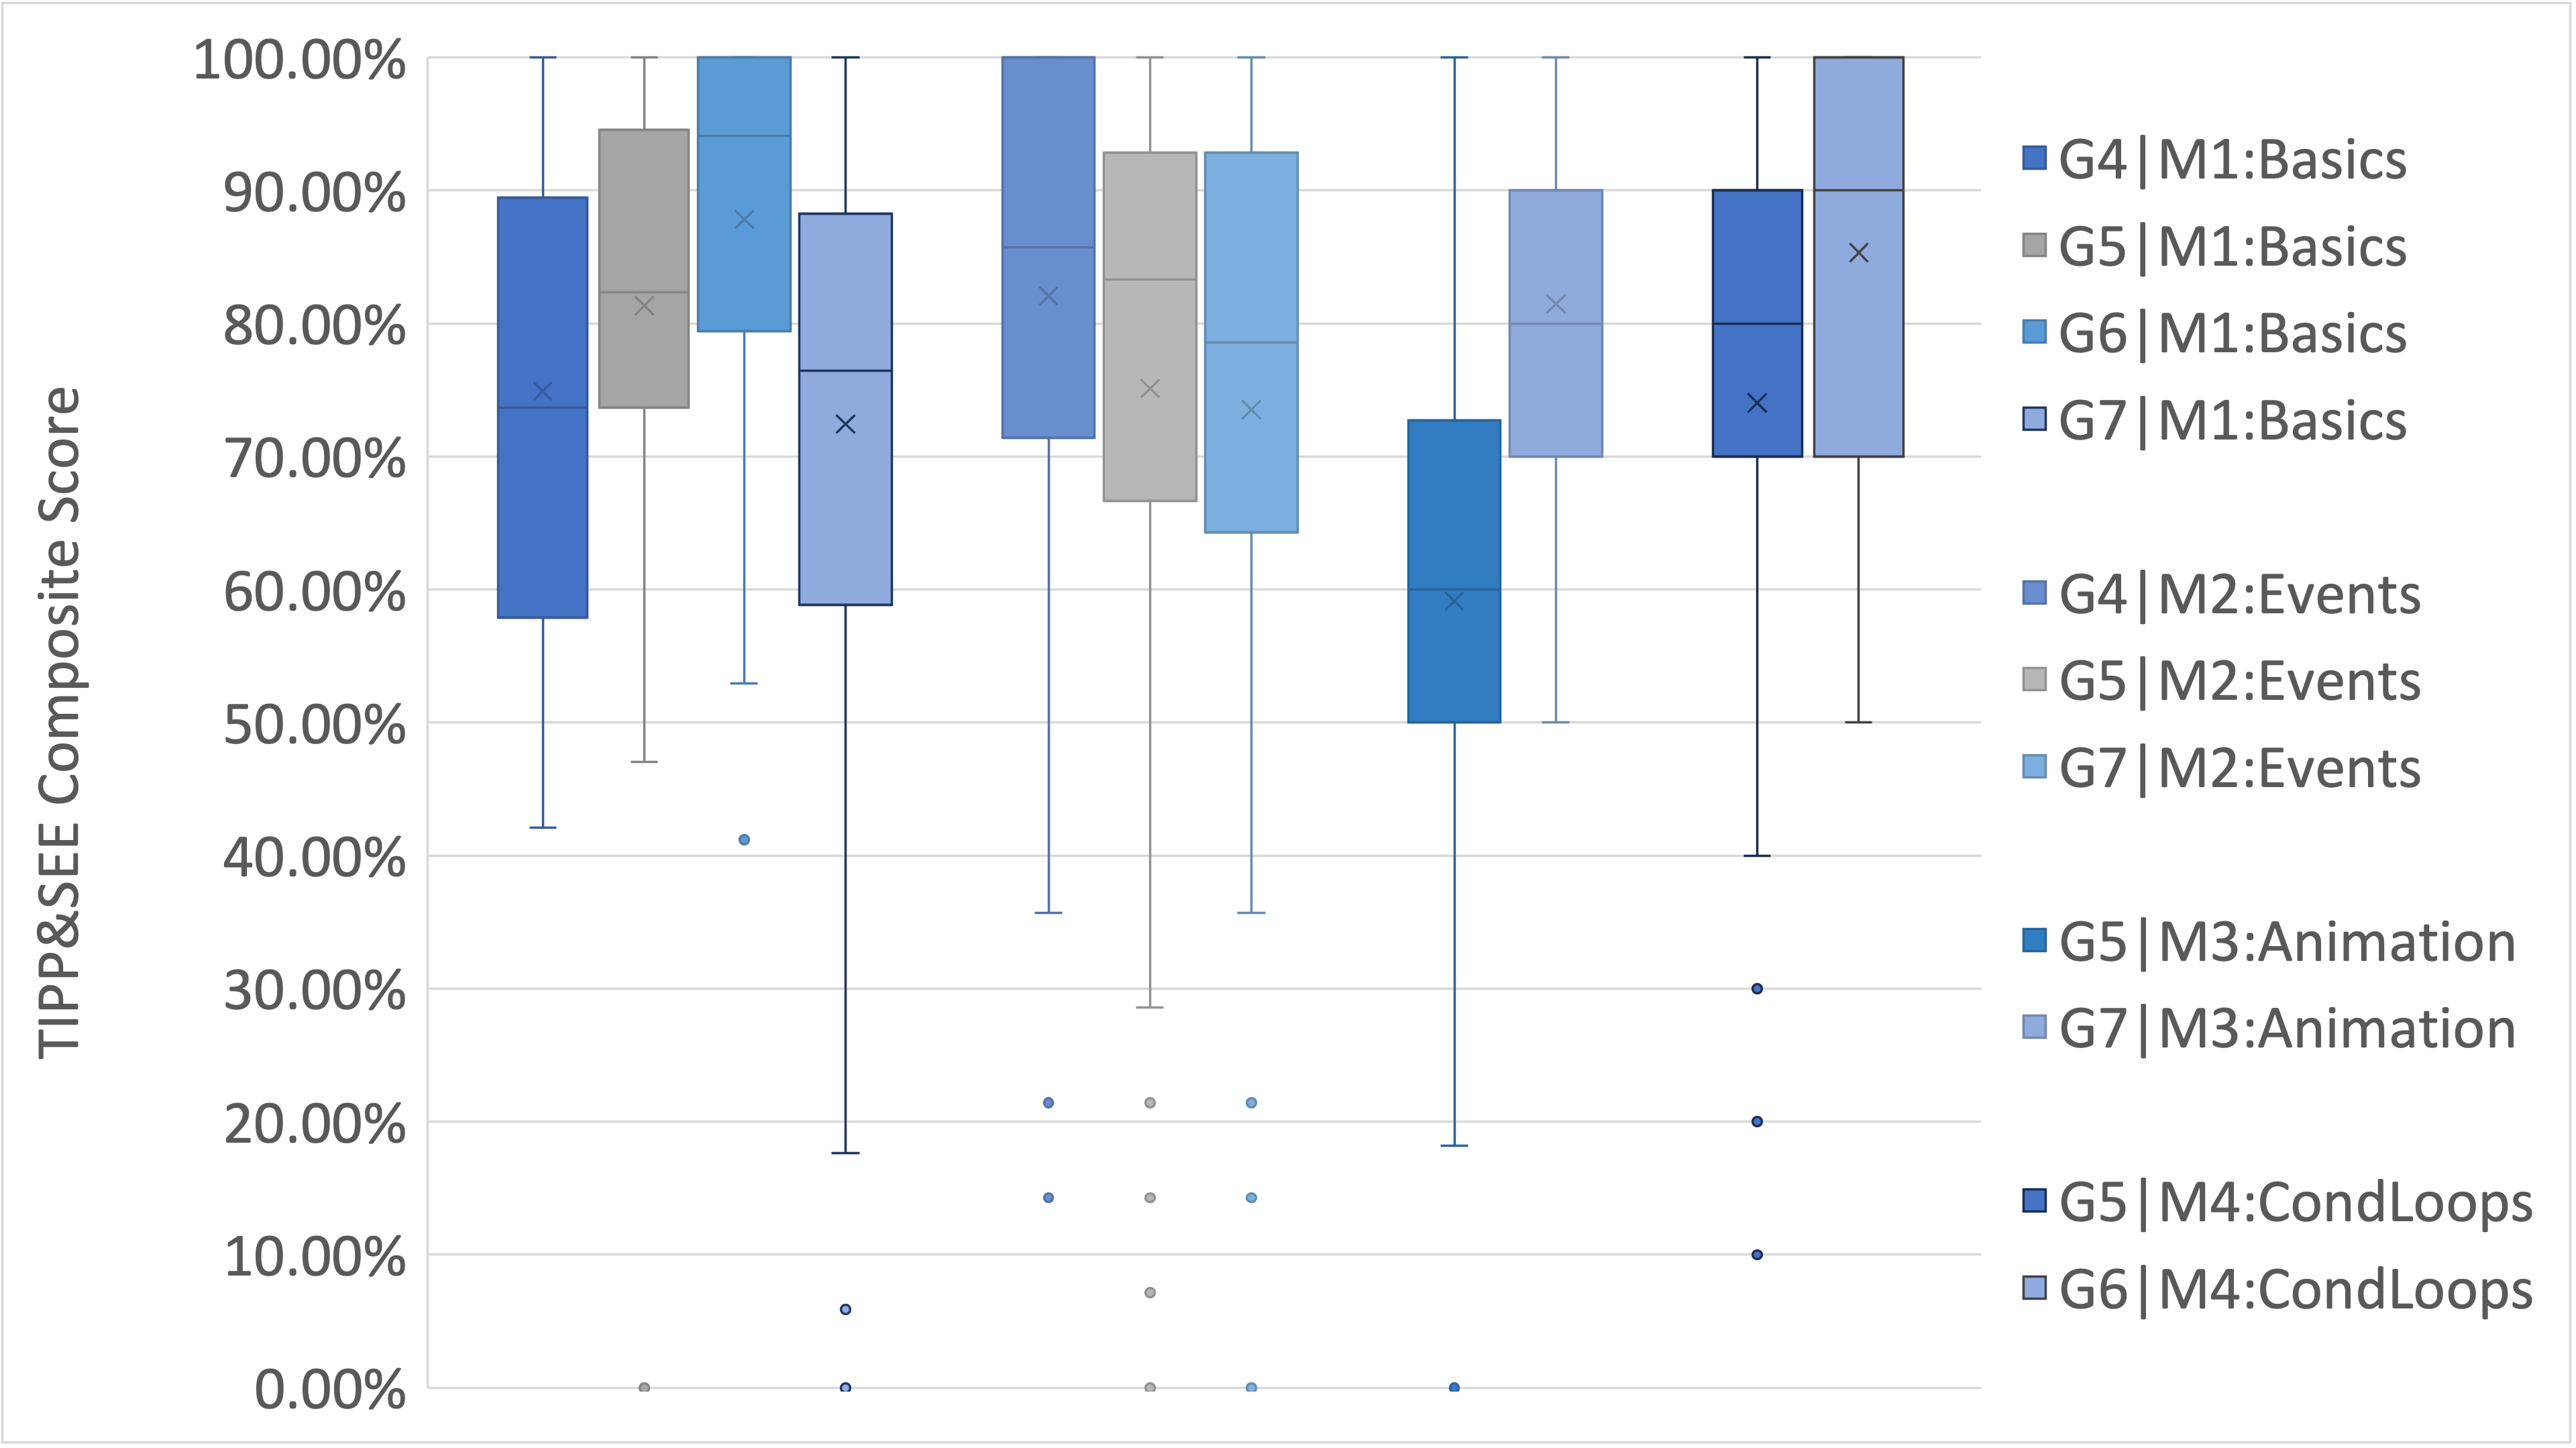
\includegraphics[width=\textwidth]{Grade.png}}
        \caption{Average \ts Worksheet Composite Scores of Students in Various Middle-School Grade Levels}
        \label{fig:grade_factors}
    \end{subfigure}
    \hfill
    \begin{subfigure}[t]{0.49\textwidth}
        \raisebox{-\height}{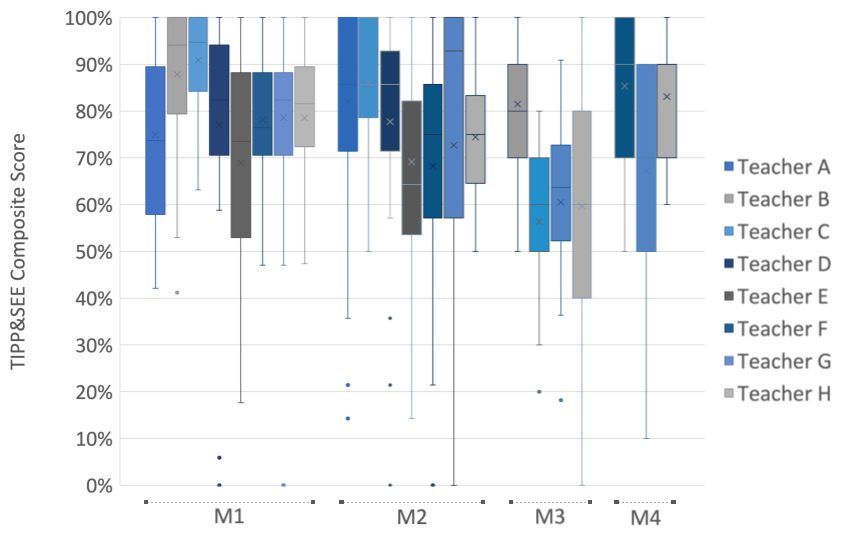
\includegraphics[width=\textwidth]{Teachers.png}}
        \caption{Average \ts Worksheet Composite Scores of Students with Different Teachers}
        \label{fig:teacher_factors}
    \end{subfigure}
    \caption{\ts Scores Compared Across Classroom-related Factors}
    \label{fig:classroom_factors}
\end{figure}



%Strand: Students were the same for M1 & M2, and different for M3 & M4. Though I don't think we should include this anymore because grade level and strand aren't independent, especially for the few classrooms who got to M3 and M4. I took a closer look at the data and the strands which had older grades had higher scores than the strands with lower grades, so we're not getting an accurate picture of what the differences between strands are; it's just a proxy for grade level.

% \begin{figure}
%      \centering
%     \begin{subfigure}[t]{0.49\textwidth}
%         \raisebox{-\height}{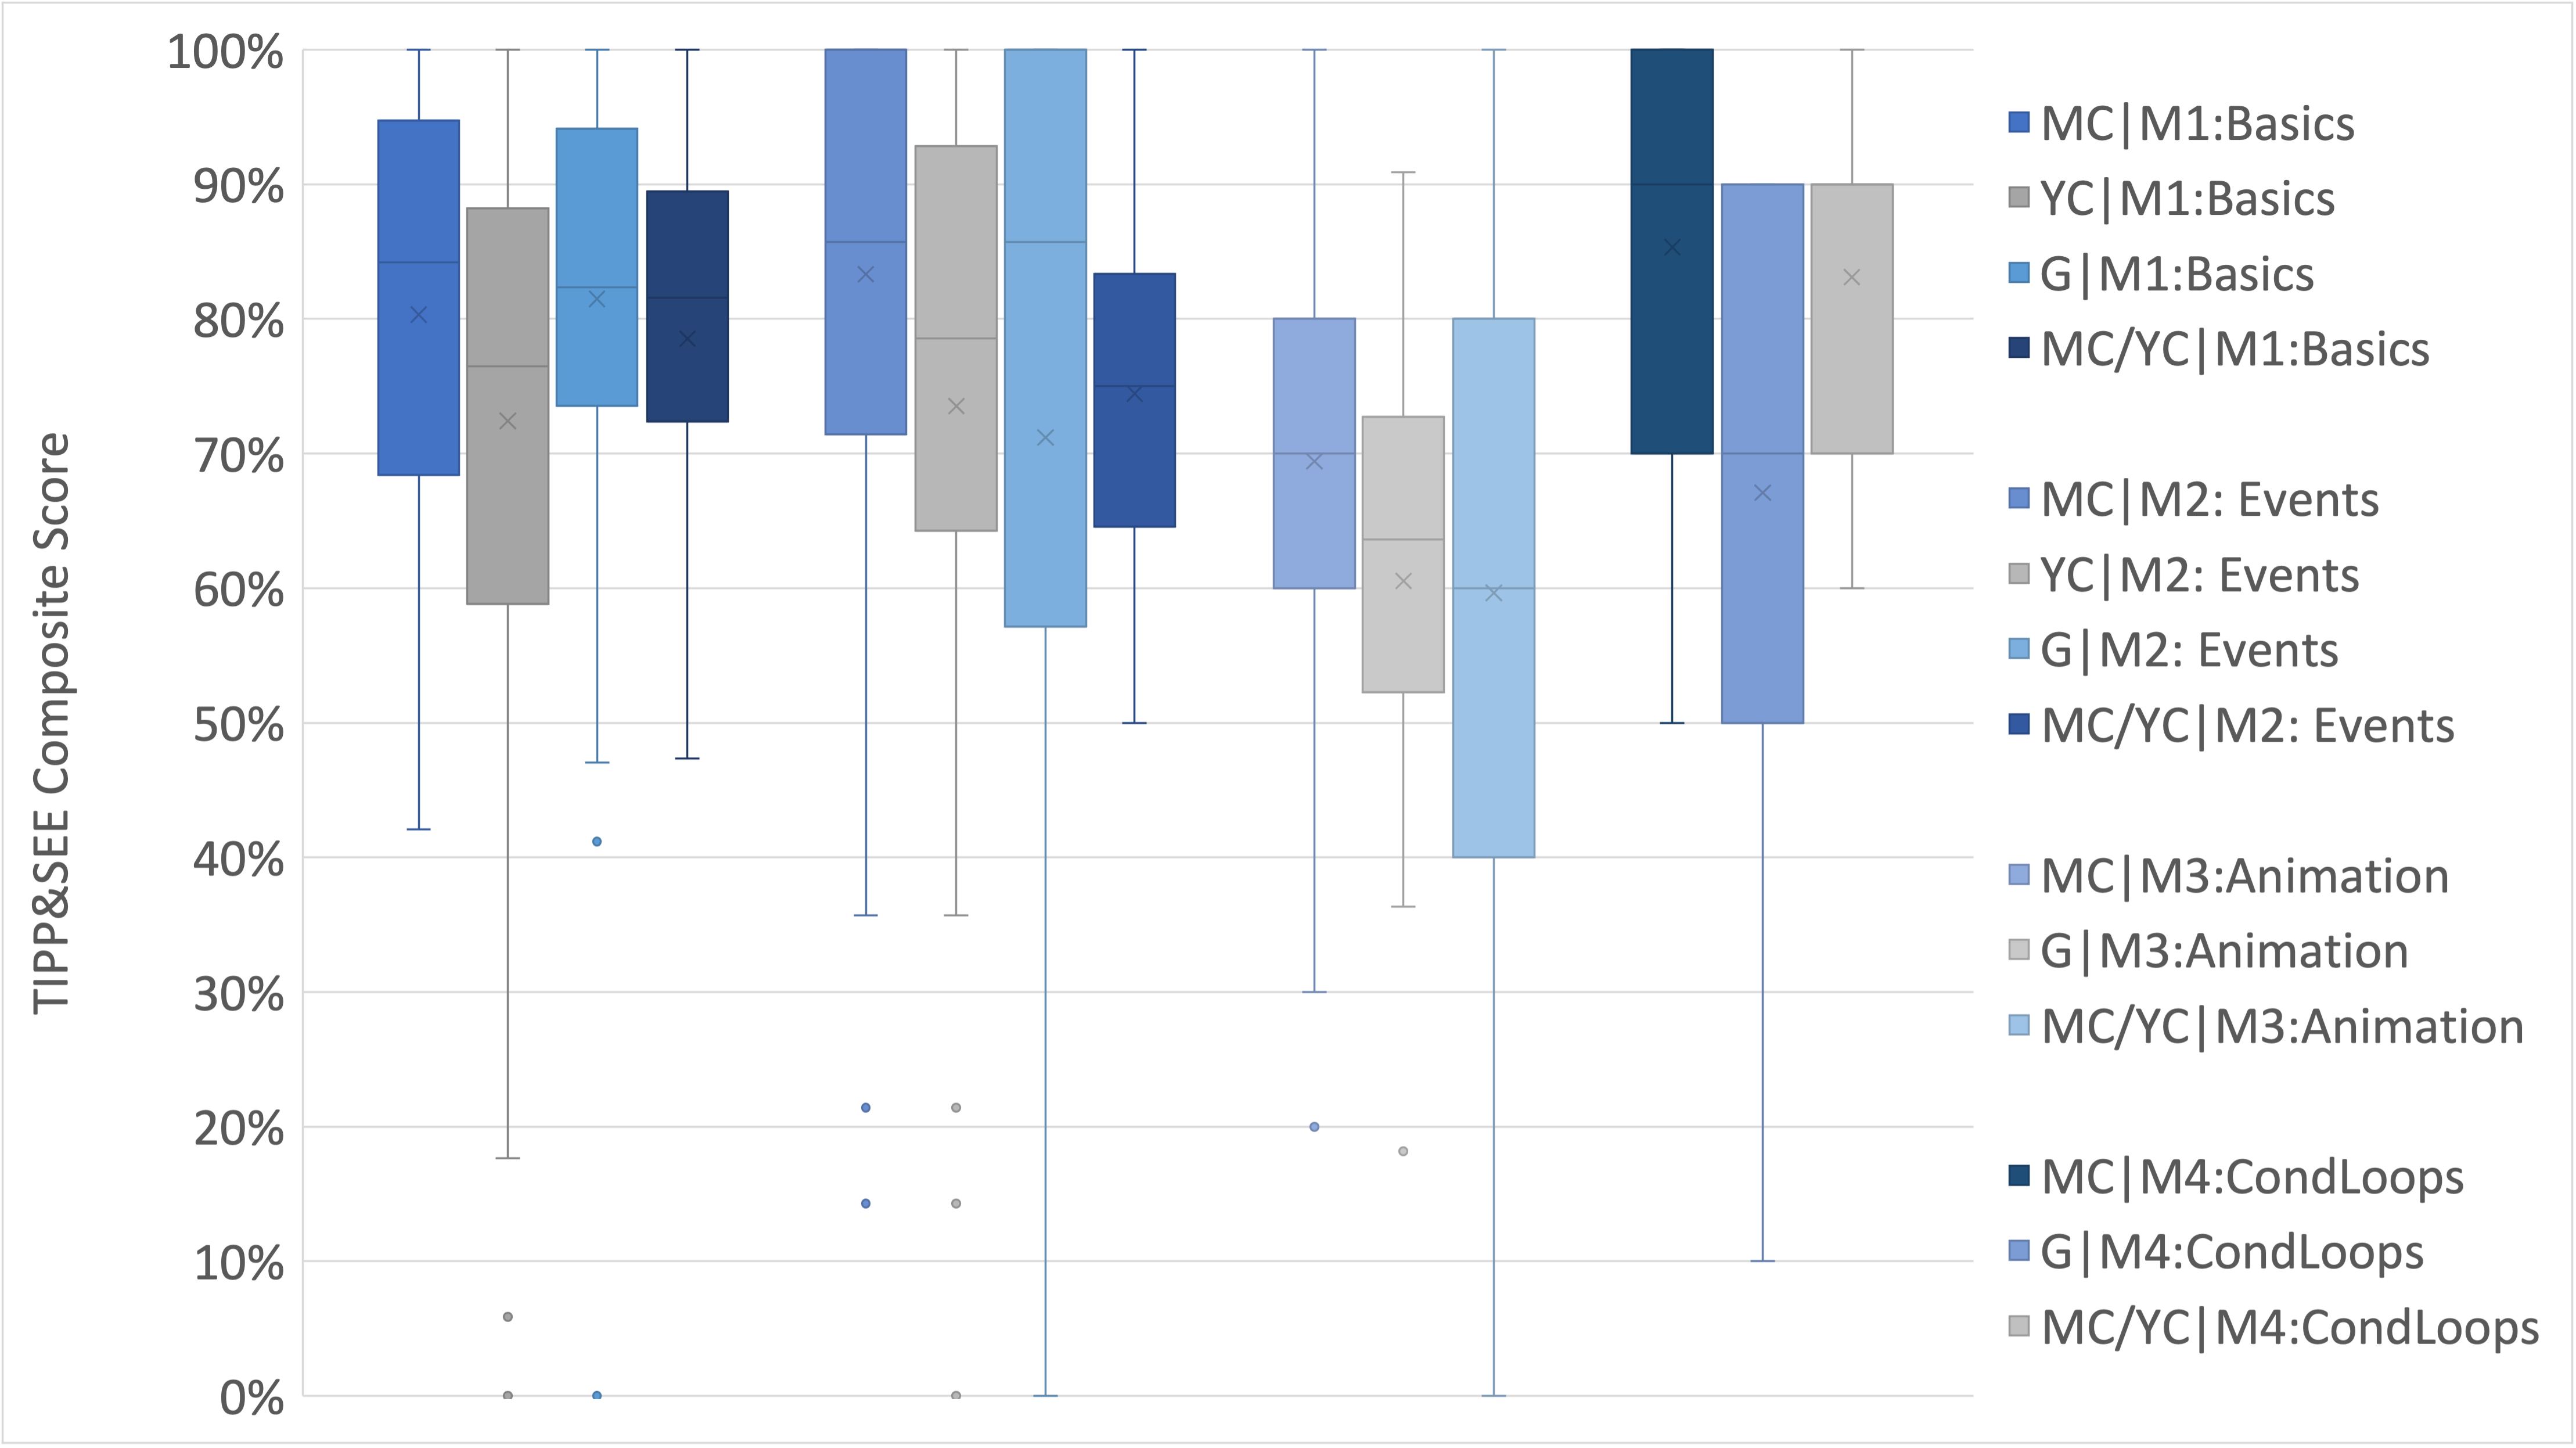
\includegraphics[width=\textwidth]{Strand.png}}
%         \caption{Distribution of \ts Composite Scores Across Strands of \scratchencore\\Note: Y-axis begins at 40\%}
%     \end{subfigure}
%     \hfill
%     \begin{subfigure}[t]{0.49\textwidth}
%         \raisebox{-\height}{\includegraphics[width=\textwidth]{Modules.png}}
%         \caption{Average \ts Worksheet Composite Scores of Students in Modules 1-4}
%     \end{subfigure}
%     \caption{\ts Scores Compared Across Curriculum-related factors}
%     \label{fig:curriculum_factors}
% \end{figure}


 
 \subsection{Student-based Factors}
 
 Next, we examined student-based factors. These are parent-reported factors about the students' struggles in mathematics and their parent-reported previous experience with programming.
 
 \stepcounter{findingnum}
 \textit{Finding \arabic{findingnum}: Students using \ts{} performed equally well on worksheets regardless of their prior struggles with mathematics or previous experience with programming.}
 
 \begin{figure}
     \centering
    \begin{subfigure}[t]{0.49\textwidth}
        \raisebox{-\height}{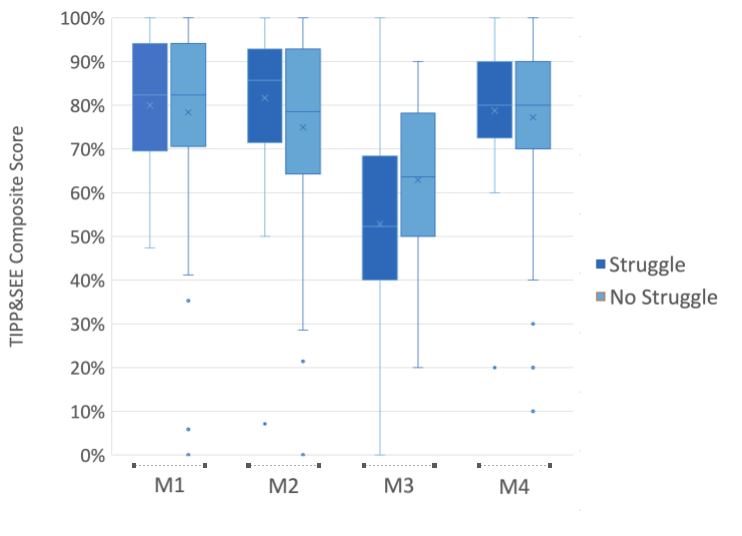
\includegraphics[width=\textwidth]{Math.png}}
        \caption{Average \ts Worksheet Composite Scores of Students who do and do not Self-Reportedly Struggle on Mathematics Homework}
    \end{subfigure}
    \hfill
    \begin{subfigure}[t]{0.49\textwidth}
        \raisebox{-\height}{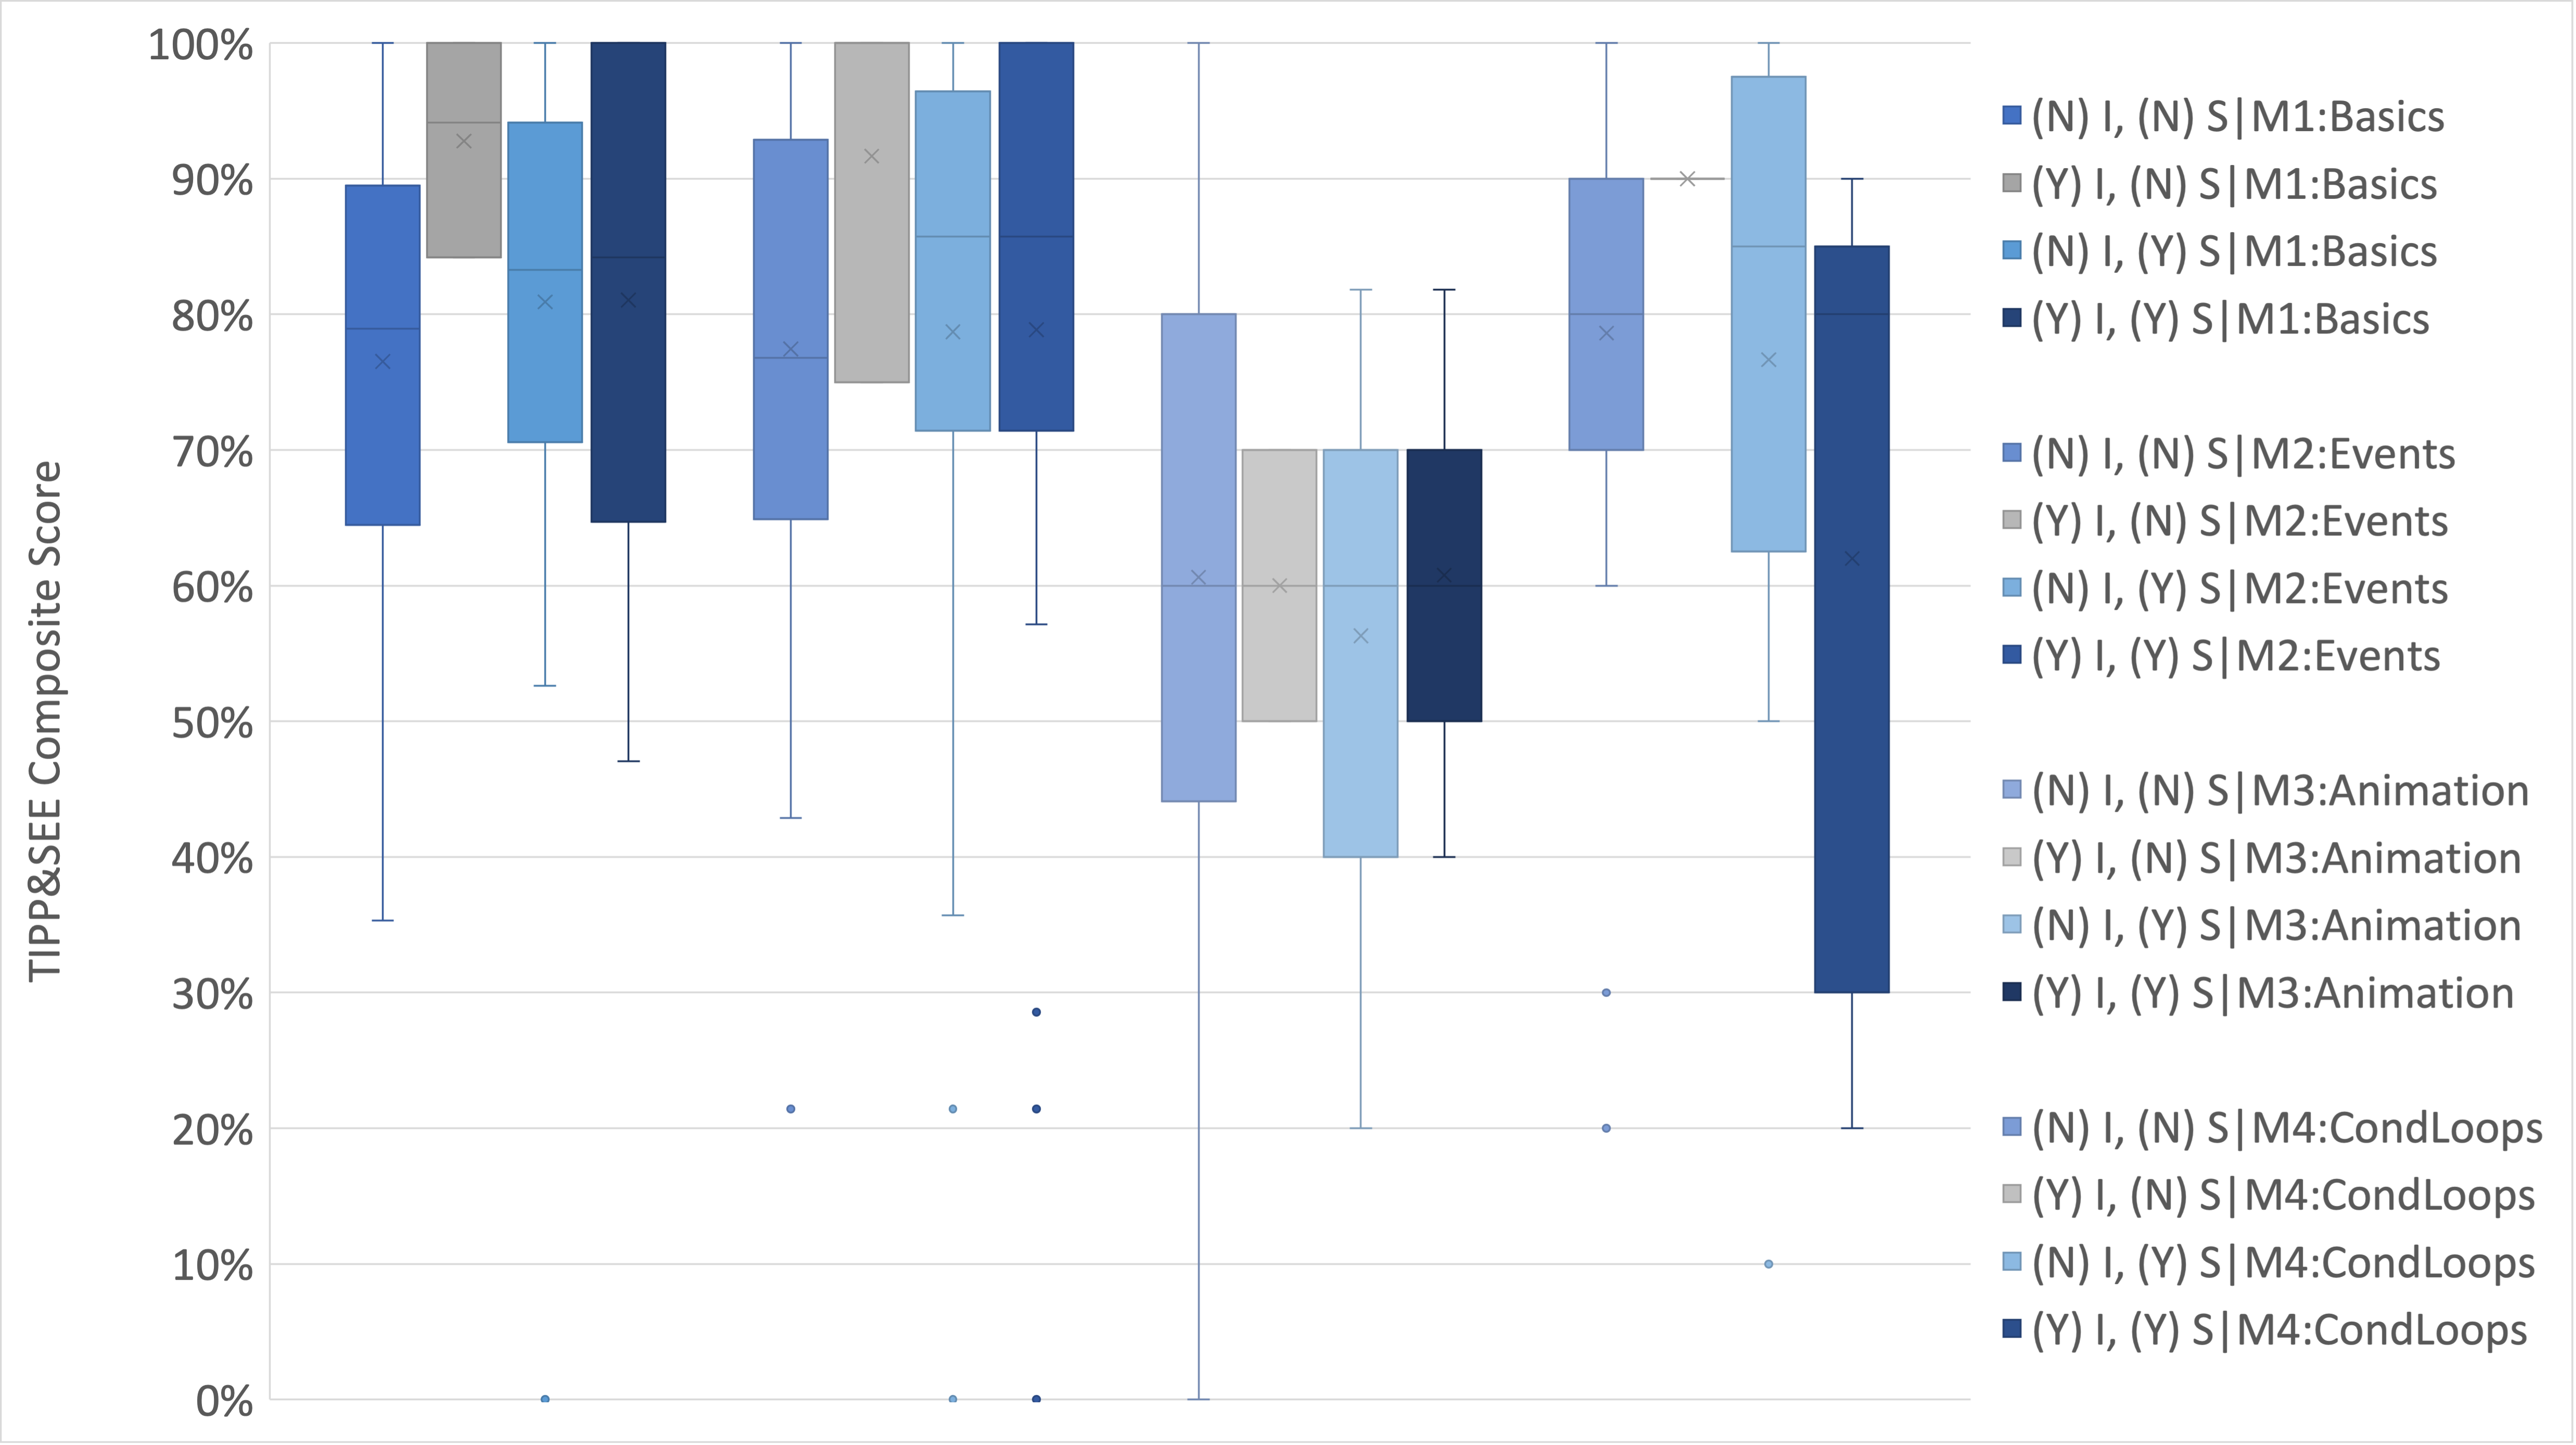
\includegraphics[width=\textwidth]{Previous_Experience.png}}
    \caption{Average \ts Worksheet Composite Scores of Students with Various Combinations of Levels of Informal and In-School Programming Experience} 
    \end{subfigure}
    \caption{\ts Scores Compared Across Levels of Previous STEM Experience}
    \label{fig:math_programming}
\end{figure}

Figure \ref{fig:math_programming} presents: (a) the average composite \ts{} worksheet scores of students whose parents indicated that the student has struggled to complete their mathematics homework in the past compared to those who did not struggle (b) the average composite scores of students stratified by their experience with programming in an informal or school setting. The average \ts{} composite score for students with no mathematics struggle was 91.66\% and the average score for those whose parents reported previous struggles in mathematics coursework was 91.23\%. Our statistical analysis showed that there was no significant difference in performance on \ts{} worksheets between students with and without math struggle in all four modules (\begin{math}M1: F(2, 147)=1.74, p=.179; M2: F(2,139)=.0552, p=.947; M3: \chi=.366, p=.545; M4: \chi=.00367, p=.952\end{math}). As for results based on prior programming experience, the average \ts{} composite score for students with no informal school or programming experience was 91.09\%. For students with informal but no school programming experience, the average was 96.16\%. For those with school but no informal programming experience, the average was 91.99\%. Finally, the average score for those with both school and informal programming experience was 92.09\%. These differences were not statistically significant(\begin{math}M1: \chi=4.32, p=.229; M2: \chi=4.54, p=.209; M3: \chi=.820, p=.845; M4: \chi=3.978, p=.264\end{math}). These results are promising and indicate that \ts{} is effective in serving as an equitable learning strategy despite students' struggles in mathematics or previous experiences as reported by their parents.

\subsection{Question-based Factors}
 \label{qb-factors}
 
Lastly, we examined worksheet-based factors. Those factors include the types of questions on the worksheet, whether the questions had a common-sense interpretation, and the position of the question within sections of the worksheet. 
 
%Lastly, we examined worksheet-based factors. Those factors include the types of questions on the worksheet, whether the questions had a real-world, common-sense, everyday interpretation, and the position of the question within sections of the worksheet. 

\stepcounter{findingnum}
\textit{Finding \arabic{findingnum}: Students attempted "Observe" and "Explore" questions more often than they did "Predict" questions. Students attempted "Observe" questions more than "Explore" questions.}

\begin{figure}
     \centering
     \begin{subfigure}[t]{0.49\textwidth}
        \raisebox{-\height}{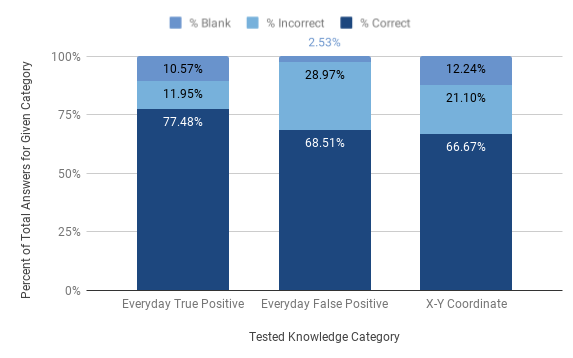
\includegraphics[width=\textwidth]{Observe_Predict_Explore_Overall.png}}
        \caption{Student Performance on 2019-2020 \ts Worksheets by Question Type}
        \label{fig:observe_predict_explore}
    \end{subfigure}
    \hfill
    \begin{subfigure}[t]{0.49\textwidth}
        \raisebox{-\height}{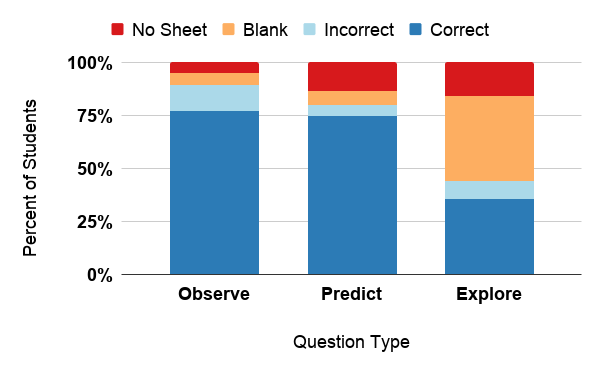
\includegraphics[width=\textwidth]{4Grade_TIPPSEE_Agg_Question.png}}
        \caption{4th Grade Student Performance on \ts Worksheets by Question Type From Previous Study}
        \label{fig:observe_predict_explore_4th}
    \end{subfigure}
    \caption{\ts Scores Compared Across Question Type}
    
\end{figure}

Figure \ref{fig:observe_predict_explore} presents the percent total of correct, incorrect, and blank student answers for each worksheet section: "Observe", "Predict", or "Explore". We found that across modules, students attempted questions within each section of the worksheet at different rates. Students were less likely to attempt and correctly answer “Predict” questions (which asked students to demonstrate a theoretical understanding of the function of blocks) and "Explore questions" (which asked students to make small modifications to existing code to demonstrate a particular concept); the difference was statistically significant (\begin{math}\chi=71.34, p<.01\end{math}). That is, students were least likely to attempt questions that required them to hypothesize about the function of a block or make changes to example code instead of following directions.

Figure \ref{fig:observe_predict_explore_4th} presents findings from previous work on 4th grade students' \ts{} behavior \cite{franklin2020exploring}. While 4th grade students in previous work and the 4th-7th grade students in this study answered "Observe" questions at a similar rate (\begin{math}\chi=2.86, p=.239\end{math}), students in this study were more likely to attempt and correctly answer "Predict" (\begin{math}\chi=70.86, p<.01\end{math}) and "Explore" questions (\begin{math}\chi=556.43, p<.01\end{math}). \hide{They found that across modules, students completed "Observe" and "Predict" questions more and answered them more accurately. A much larger portion of the "Explore" questions were left unanswered.}

\stepcounter{findingnum}
\textit{Finding \arabic{findingnum}: Students were more correct on "Observe" questions than "Predict" and "Explore" questions.} 

Students answered “Predict” and “Explore” questions with comparable correctness, while answering “Observe” questions correctly more than the other two categories. Additionally, "Observe" questions had the fewest incorrect answers while "Explore" questions had the most incorrect answers. As seen in Figure \ref{fig:observe_predict_explore}, "Observe" questions were answered correctly 79.79\% of the time, incorrectly 13.43\% of the time, and left blank 6.78\% of the time. 73.24\% of "Predict" questions were answered correctly, 15.73\% incorrectly, and 11.02\% were left blank. Finally, 73.64\% of "Explore" questions were answered correctly, 18.66\% incorrectly, and 7.70\% were left blank.%say something about these observations holding across the strands that students used or other large-scale observations of students’ attempts. This could be characteristics of questions such as multiple choice/circling etc

\stepcounter{findingnum}
\textit{Finding \arabic{findingnum}: Students are more likely to answer questions and to do so accurately when the block or concept in question has a real-world, common-sense, everyday interpretation.}

Figure \ref{fig:everyday_school} illustrates the differences in answer correctness and answer rate for \ts{} worksheet questions when divided by whether what they were asking students about a concept which matched with its real-world interpretation (Everyday True Positive), did not match with its real-world interpretation (Everyday False Positive), or did not have a straightforward real-world interpretation to begin with and relied primarily on knowledge gained in school settings (School). The figure displays the percent of each response type (correct, incorrect, and blank) in each category. We found a statistically-significant association between response type and the type of knowledge used for a concept (\begin{math}\chi=56.25, p<.01\end{math}). Everyday True Positive questions and Everyday False Positive questions were answered correctly 77.10\% and 80.84\% of the time, respectively, whereas only 68.97\% of School questions were answered correctly. Further, students left 13.13\% of School questions blank, 3.9\% more than Everyday False Positive questions (which were left blank 9.23\% of the time) and 5.46\% more than Everyday True Positive questions (left blank 7.67\% of the time). Additionally, students answered more School questions (17.91\%) incorrectly than Everyday True Positive (15.23\%) and Everyday False Positive (9.93\%) questions.

This data shows that questions testing blocks or concepts that are connected to a school-knowledge meaning are the most likely to be skipped or answered incorrectly by middle grade students when engaging with the \ts{} learning strategy. This behavior may occur because students are associating those blocks or concepts with concepts they have learned in other subjects. Therefore, students who may be less comfortable with certain blocks or concepts, such as variables or blocks that ask students to use the coordinate system.

% this is the "so what" but maybe it belongs in the discussion? I put it both places to decide where it goes better:

%\ts and \scratchencore were created and this study was conducted in order to provide equitable access to intermediate computer science education to middle grade students. In order to do so, it is important to understand if the \ts worksheets impacts student success on theoretical and abstract concepts. In finding 0, we demonstrate that parent-reported previous coursework in programming and mathematics does not impact student engagement or success. In this finding, however, we show that the \ts worksheets that include concepts from previous coursework in mathematics and computer science do impact student engagement as they are the most frequently skipped and the most frequently answered incorrectly. This may be indicative of middle school students' perceptions of the relevance of other coursework to their computer science education. Further research could involve asking students if they perceived the "School" questions as implying that their performance in their other coursework was relevant to their success in their computer science course work. This pre-judgement may cause students to simply not answer the question, if they feel it appears to require knowledge from other coursework.

\stepcounter{findingnum}
\textit{Finding \arabic{findingnum}: The position of a question within a section had an effect on whether or not students were likely to attempt it as well as their correctness.} 

\begin{figure}
     \centering
     \begin{subfigure}{0.49\textwidth}
        \raisebox{-\height}{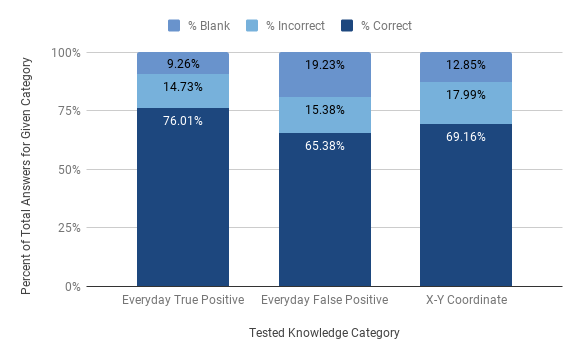
\includegraphics[width=\textwidth]{E_EF_S.png}}
        \caption{Student Performance on 2019-2020 \ts Worksheets by Everyday True Positive, Everyday False Positive, and School-based Knowledge Categorization}
        \label{fig:everyday_school}
    \end{subfigure}
    \begin{subfigure}{0.49\textwidth}
        \raisebox{-\height}{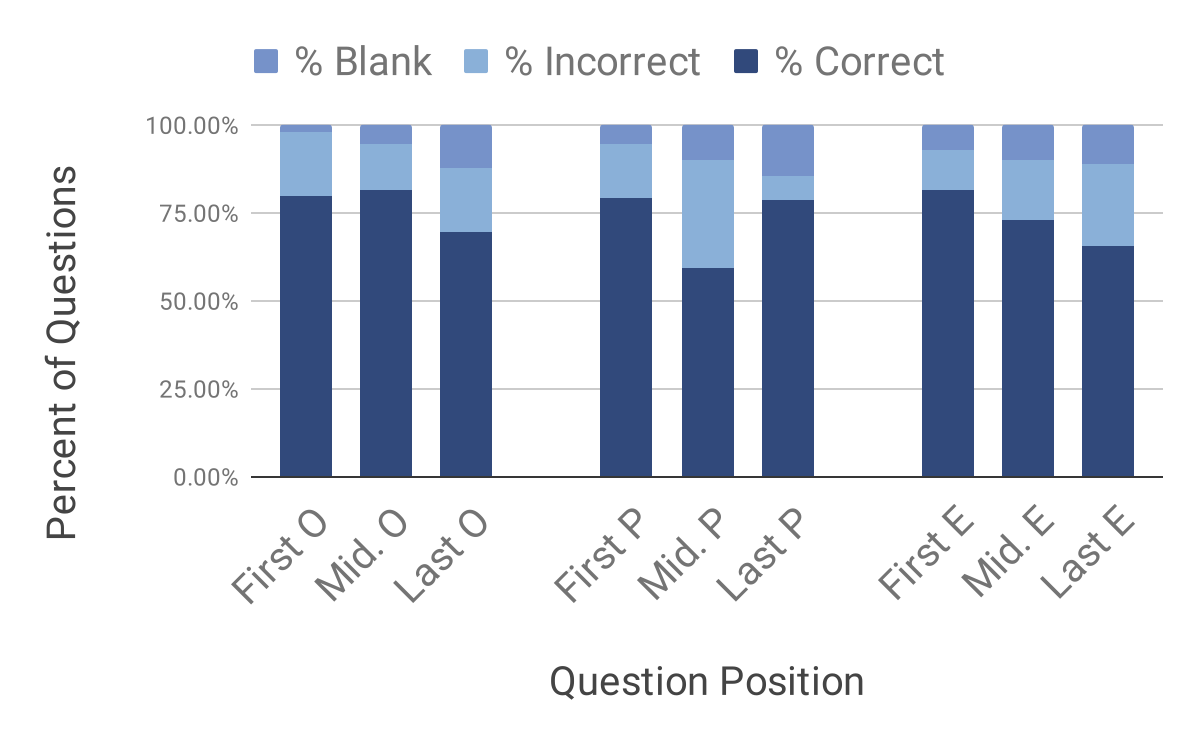
\includegraphics[width=\textwidth]{Position.png}}
        \caption{Average Worksheet Performance by Position in Section on 2019-2020 \ts Worksheets}
        \label{fig:position_es}
    \end{subfigure}
    
    \caption{Student Performance Compared Across Question Position and Question Knowledge-type}
\end{figure}

In Figure ~\ref{fig:position_es}, three lines are shown: correct (percent of attempted questions answered correctly), incorrect (percent of attempted questions answered incorrectly), and blank (percent of questions not attempted) as a function of the position of a question within a section of the worksheet, being the first, middle or last question in a given section. The students tended to attempt fewer questions as they progressed through each section, and the percentage of correct answers decreased through each section (\begin{math}\chi=76.06, p<.01\end{math}). There was similar percentage of incorrect answers from the first to the last question in the sections.

In the "Observe" section there were not any noticeable trends in the percentage of correct or incorrect answers from the first question to the last question. However, there was an increase in blank answers from the first to the last question (first: 5.31\%, middle: 9.81\%, last: 14.50\%). Similarly, we did not observe any noticeable trends in the percentage of correct or incorrect answers in the "Predict" sections. However, there was an increase from 5.31\% to 14.50\% in blank questions for the questions in the "Predict" section.

The position of a question had the strongest impact on answer correctness in the "Explore" section.  For this section, the final section of the worksheets, the percentage of correct answers changed from 81.22\% on the first question to 65.83\% on the last question. In this section, students incorrectly answered twice as many questions at the end of the section as they did at the start of the section (11.64\% to 23.28\%). Additionally, there was an increase in blank answers (first: 7.16\%, middle: 10.00\%, last: 10.94\%).

Despite there being no clear trend in incorrectness/correctness with respect to question position in the individual "Observe" and "Predict" sections, there was an increase in the average percentage of correct answers from the first to last question in all sections. Additionally, the rate of blankness rose steadily from the first to the middle through the last question of all three sections. These findings may be due to the students becoming tired of answering questions from the first to last question in the sections.

\subsection{Correlations between Projects and Worksheets}

\stepcounter{findingnum}
\textit{Finding \arabic{findingnum}: There was very little correlation between \ts{} worksheet score and project score.}

Figures \ref{fig:avg_modify} and \ref{fig:avg_create} display the correlation between the average of students' scores in \ts{} and the average of students' scores in their Modify and Create projects, respectively. The correlation is low for both the Modify (\begin{math}R^2 = 0.015\end{math}) and Create (\begin{math}R^2 = 0.009\end{math}) projects. The correlation between the Modify project and \ts{} score was slightly higher. 

\begin{figure}
     \centering
     \begin{subfigure}{0.49\textwidth}
        \raisebox{-\height}{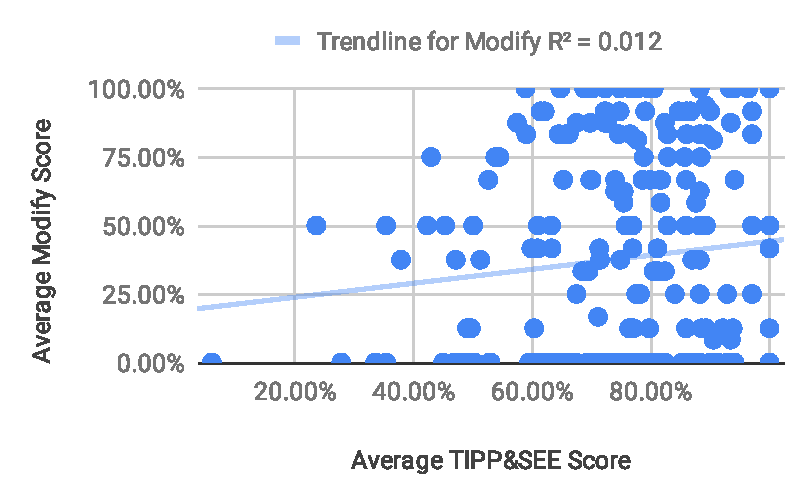
\includegraphics[width=\textwidth]{Average Modify vs. TIPP&SEE.pdf}}
        \caption{Average Modify scores vs. \ts{} scores}
        \label{fig:avg_modify}
    \end{subfigure}
    \begin{subfigure}{0.49\textwidth}
        \raisebox{-\height}{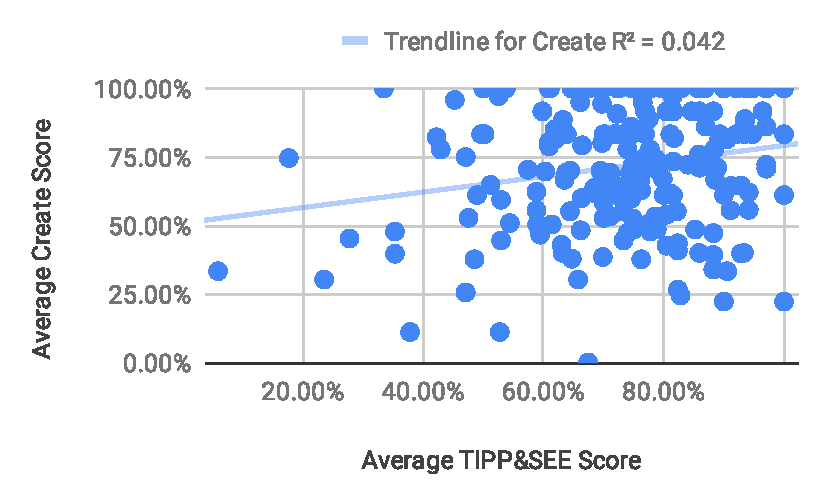
\includegraphics[width=\textwidth]{Average Create vs. TIPP&SEE.pdf}}
        \caption{Average Create scores vs. \ts{} scores}
        \label{fig:avg_create}
    \end{subfigure}
    
    \caption{Average Modify and Create scores vs. \ts{} scores}
\end{figure}


} % end of hide old results

%\section{Results}

In this work, we examine the effectiveness of \ts with middle grade students. Our analysis focused on the students' performance and completeness on the worksheets as well as the scores of their Modify and Create Projects. We explored the effects of various internal (student-based), external (environment-based), and question-specific factors on student interaction with the worksheets, and how their \ts{} scores correlated with their project scores. This resulted in four sets of results. We then synthesize our findings with respect to each other and our research questions in Section \ref{sec:discussion}.

\newcounter{findingnum}

\subsection{Environment-based Factors}

%We begin our presentation of findings with overall results highlighting the effectiveness of \ts as a learning strategy for middle grade students, before then exploring particular behaviors noticed in students engaging with the strategy. The overall results are broken into two subfindings: the effects of student-based factors (i.e. parent-reported previous relevant academic and extra-curricular experience) and environment-based factors (i.e. learning environment and curriculum structure).
First, we discuss the environmental factors. These factors include the students' grade levels, teachers, and the modules of the curriculum.

\stepcounter{findingnum}
\textit{Finding \arabic{findingnum}: Students using \ts{} performed similarly well in all grade levels across two \scratchencore{} modules but overall, they differed in performance based on module and teacher.} 

Figure \ref{fig:classroom_factors} illustrates the difference in \ts{} worksheet performance by grade level and teacher. The average \ts{} composite score for grade 4 students was 91.24\%, 90.84\% for grade 5, 94.53\% for grade 6, and 90.90\% for grade 7. For Module 2 and Module 4, students across all grade levels completed the worksheets with similar correctness ($M2: F(2,209)=.0158, p=.984; M4:\chi=3.391, p=.0656$). In contrast, for Module 1 and 3, grade level was linked to worksheet correctness ($M1: F(3, 255)=4.30, p<.01, \eta^2=.0482; M3:\chi=23.79, p<.01, \eta^2=.0747$). Post-hoc comparisons for Module 1 reveal significant differences in correctness between 6th graders and both 4th and 7th graders ($p<.05$). For Module 3, 7th graders performed better than 5th graders ($p<.01$). It is interesting to note that while there was a difference between Module 1 and Module 3, there were no differences between 5th and 6th graders for Module 4.

Next, we examined the results when stratified by the particular modules within the curriculum, allowing us to observe whether certain elements of the curriculum itself (considered to be an environmental factor) affected student success. The results of this stratification by curriculum factors are provided in Figure \ref{fig:curriculum_factors}. The average composite score for Module 1 was 91.12\%, 91.97\% for Module 2, 88.78\% for Module 3, and 91.88\% for Module 4. Our statistical analysis revealed that student worksheet correctness was different across the different modules ($F(3,668)=4.10, p<0.01, \eta^2=.0181$).

Finally, we investigated whether there was a difference in student performance on the worksheets based on the teachers (Figure \ref{fig:teacher_factors}). Average composite scores by teacher ranged from 88.75\% to 93.64\%, with a median of 91.62\% and a standard deviation of 1.86\%. For all modules, the teacher was significantly linked to worksheet correctness ($M1: \chi=40.52, p<.01, \eta^2=.112; M2: \chi=13.10, p<.05, \eta^2=.0235, M3: \chi=29.85, p<.05, \eta^2=.0886, M4: \chi=9.50, p<.01, \eta^2=.0247$). This result echos previous findings on student performance using \ts \cite{franklin2020analysis}.

\begin{figure}
    \centering
    \includegraphics[width=.5\textwidth]{Modules.png}
    \caption{\ts Scores Compared Across Modules}
    \label{fig:curriculum_factors}
\end{figure}

\begin{figure}
     \centering
    \begin{subfigure}[t]{0.49\textwidth}
        \raisebox{-\height}{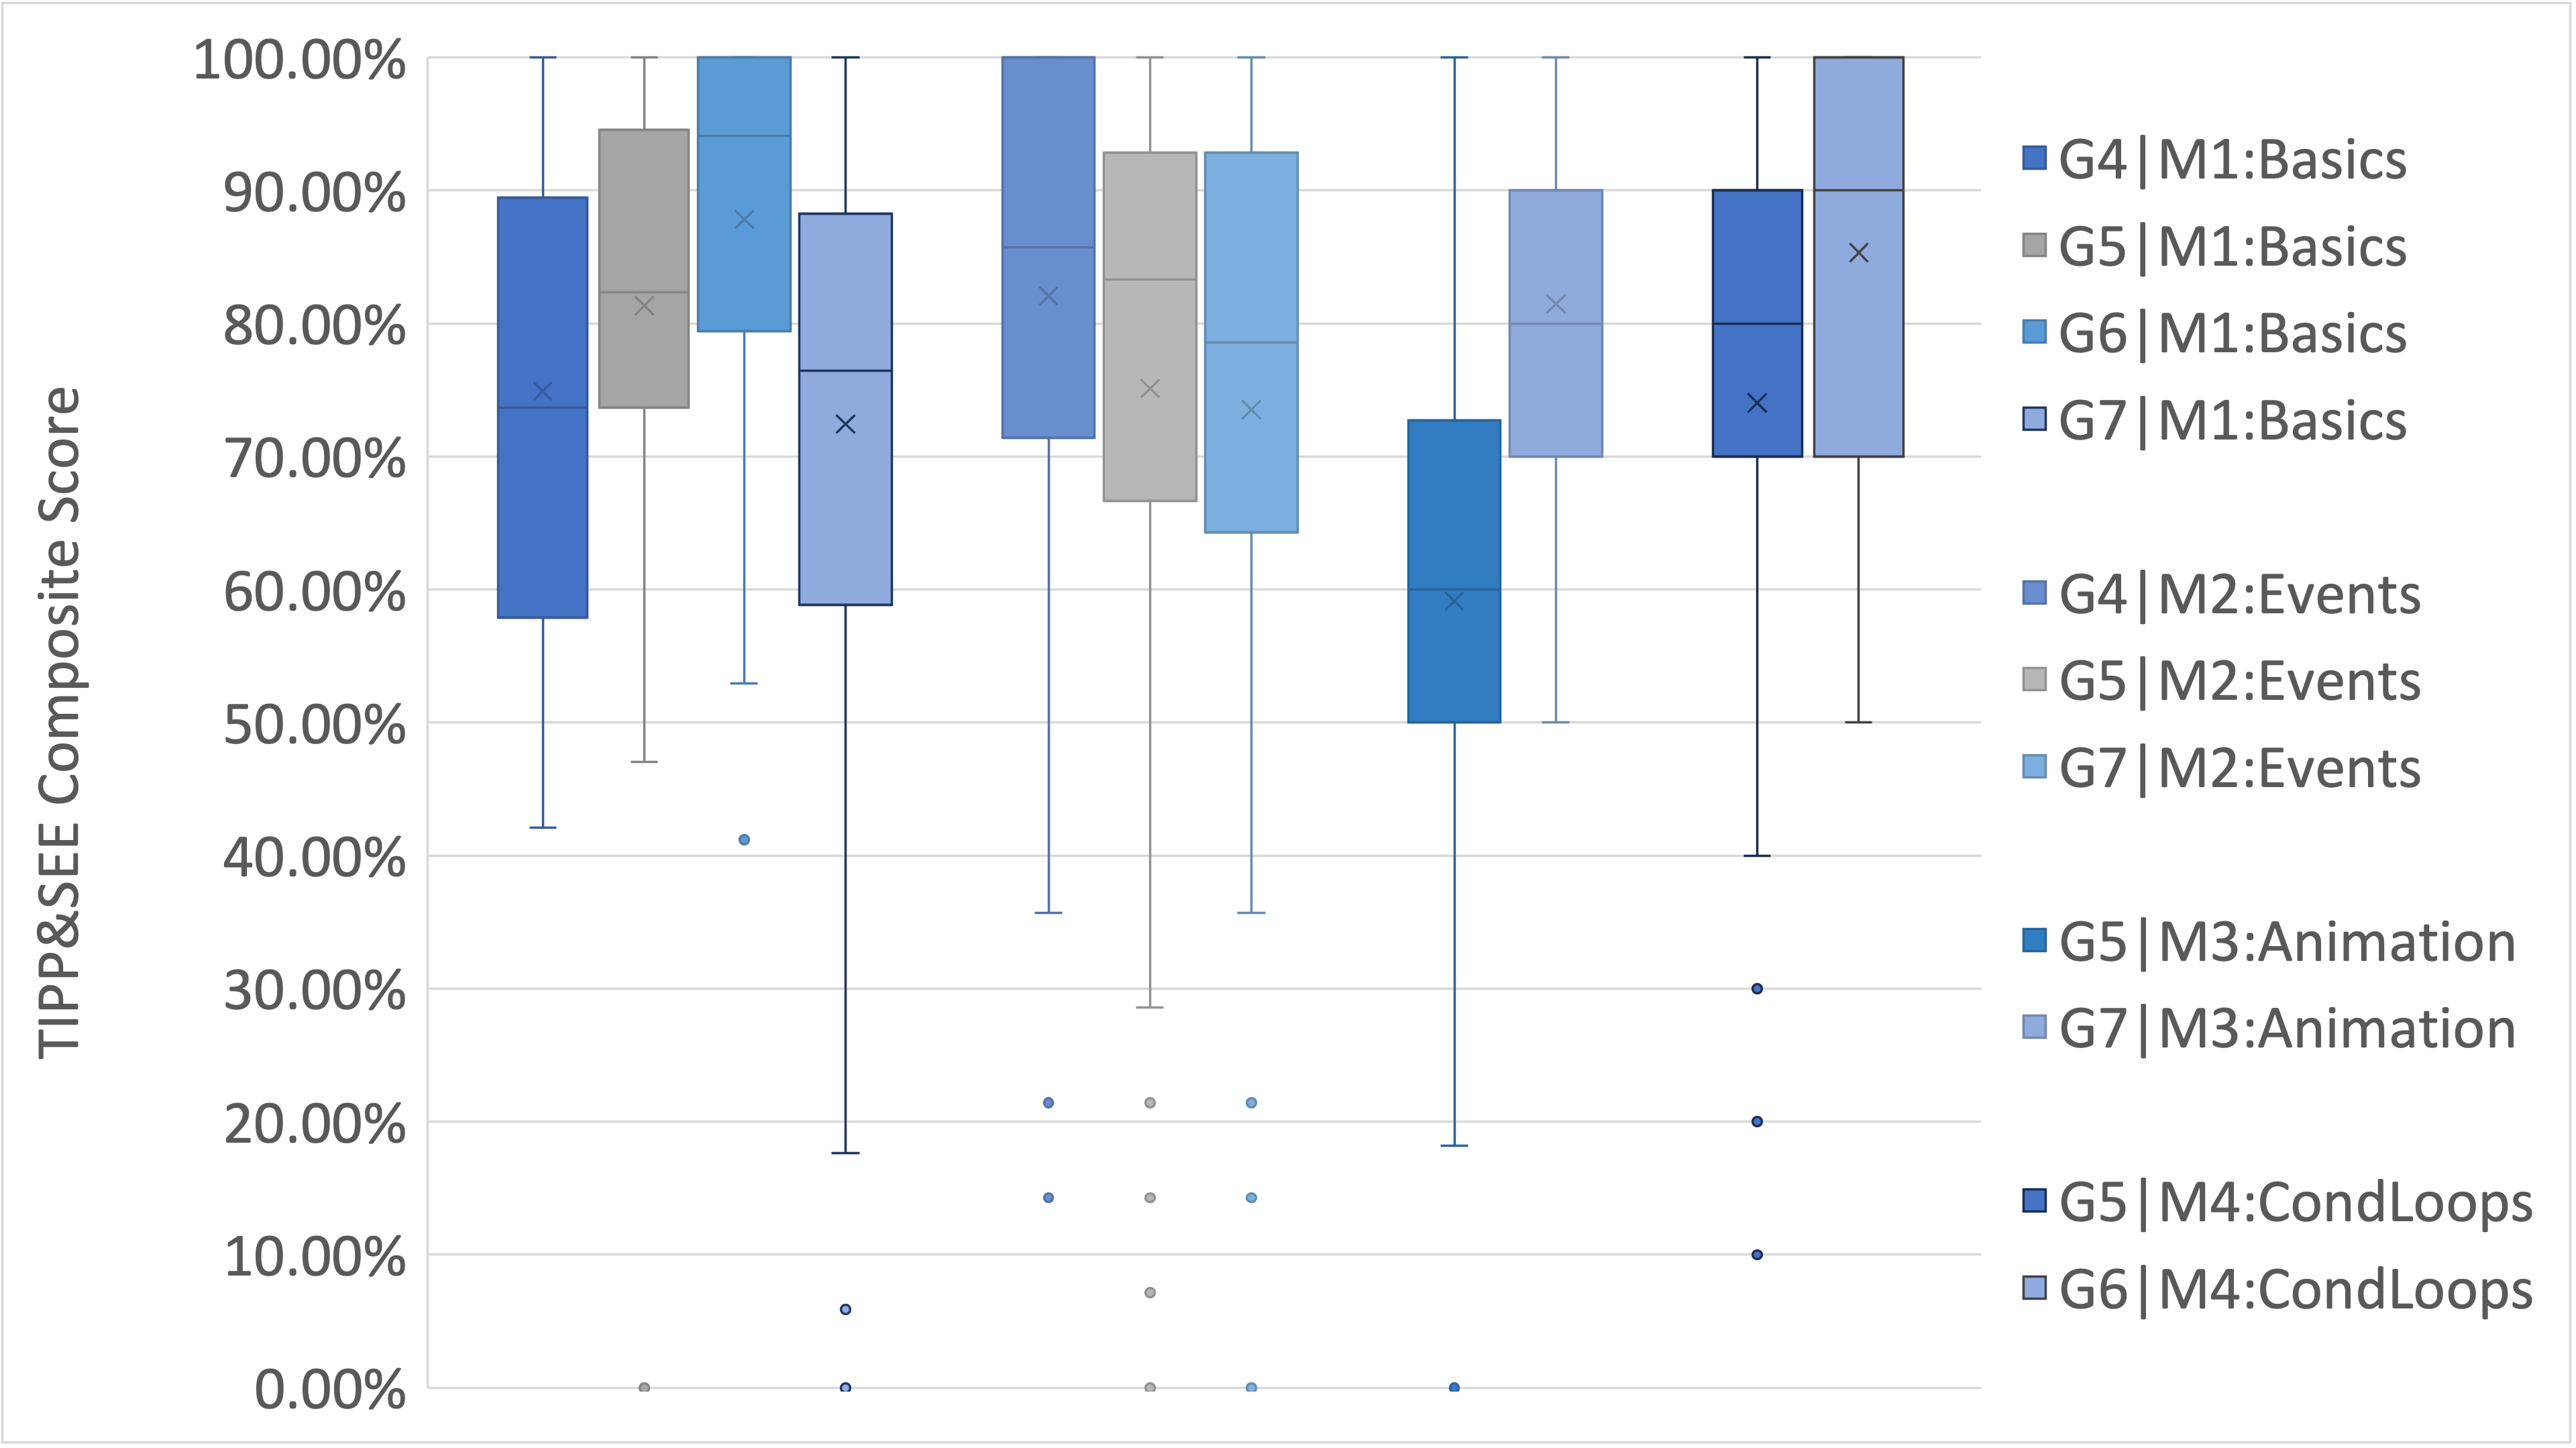
\includegraphics[width=\textwidth]{Grade.png}}
        \caption{Average \ts Worksheet Composite Scores of Students in Various Middle-School Grade Levels}
        \label{fig:grade_factors}
    \end{subfigure}
    \hfill
    \begin{subfigure}[t]{0.49\textwidth}
        \raisebox{-\height}{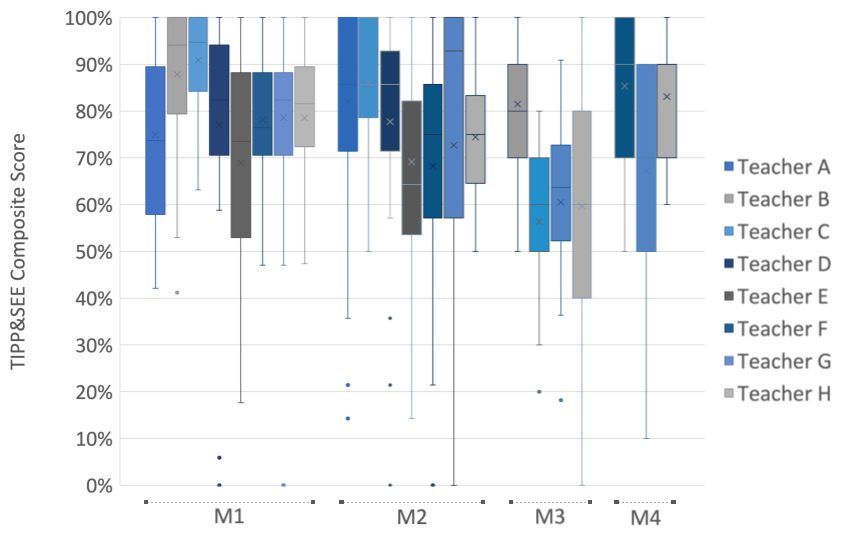
\includegraphics[width=\textwidth]{Teachers.png}}
        \caption{Average \ts Worksheet Composite Scores of Students with Different Teachers}
        \label{fig:teacher_factors}
    \end{subfigure}
    \caption{\ts Scores Compared Across Classroom-related Factors}
    \label{fig:classroom_factors}
\end{figure}



%Strand: Students were the same for M1 & M2, and different for M3 & M4. Though I don't think we should include this anymore because grade level and strand aren't independent, especially for the few classrooms who got to M3 and M4. I took a closer look at the data and the strands which had older grades had higher scores than the strands with lower grades, so we're not getting an accurate picture of what the differences between strands are; it's just a proxy for grade level.

% \begin{figure}
%      \centering
%     \begin{subfigure}[t]{0.49\textwidth}
%         \raisebox{-\height}{\includegraphics[width=\textwidth]{Strand_Boxplot.png}}
%         \caption{Distribution of \ts Composite Scores Across Strands of \scratchencore\\Note: Y-axis begins at 40\%}
%     \end{subfigure}
%     \hfill
%     \begin{subfigure}[t]{0.49\textwidth}
%         \raisebox{-\height}{\includegraphics[width=\textwidth]{Modules.png}}
%         \caption{Average \ts Worksheet Composite Scores of Students in Modules 1-4}
%     \end{subfigure}
%     \caption{\ts Scores Compared Across Curriculum-related factors}
%     \label{fig:curriculum_factors}
% \end{figure}


 
 \subsection{Student-based Factors}
 
 Next, we examined student-based factors. These are parent-reported factors about the students' struggles in mathematics and their parent-reported previous experience with programming.
 
 \stepcounter{findingnum}
 \textit{Finding \arabic{findingnum}: Students using \ts{} performed equally well on worksheets regardless of their parent-reported mathematics struggles or previous experience with programming.}
 
 \begin{figure}
     \centering
    \begin{subfigure}[t]{0.49\textwidth}
        \raisebox{-\height}{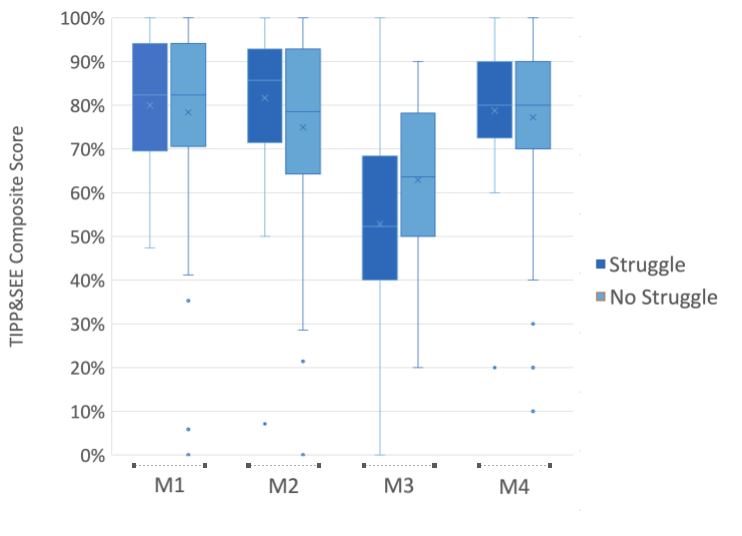
\includegraphics[width=\textwidth]{Math.png}}
        \caption{Average \ts Worksheet Composite Scores of Students who do and do not Self-Reportedly Struggle on Mathematics Homework}
    \end{subfigure}
    \hfill
    \begin{subfigure}[t]{0.49\textwidth}
        \raisebox{-\height}{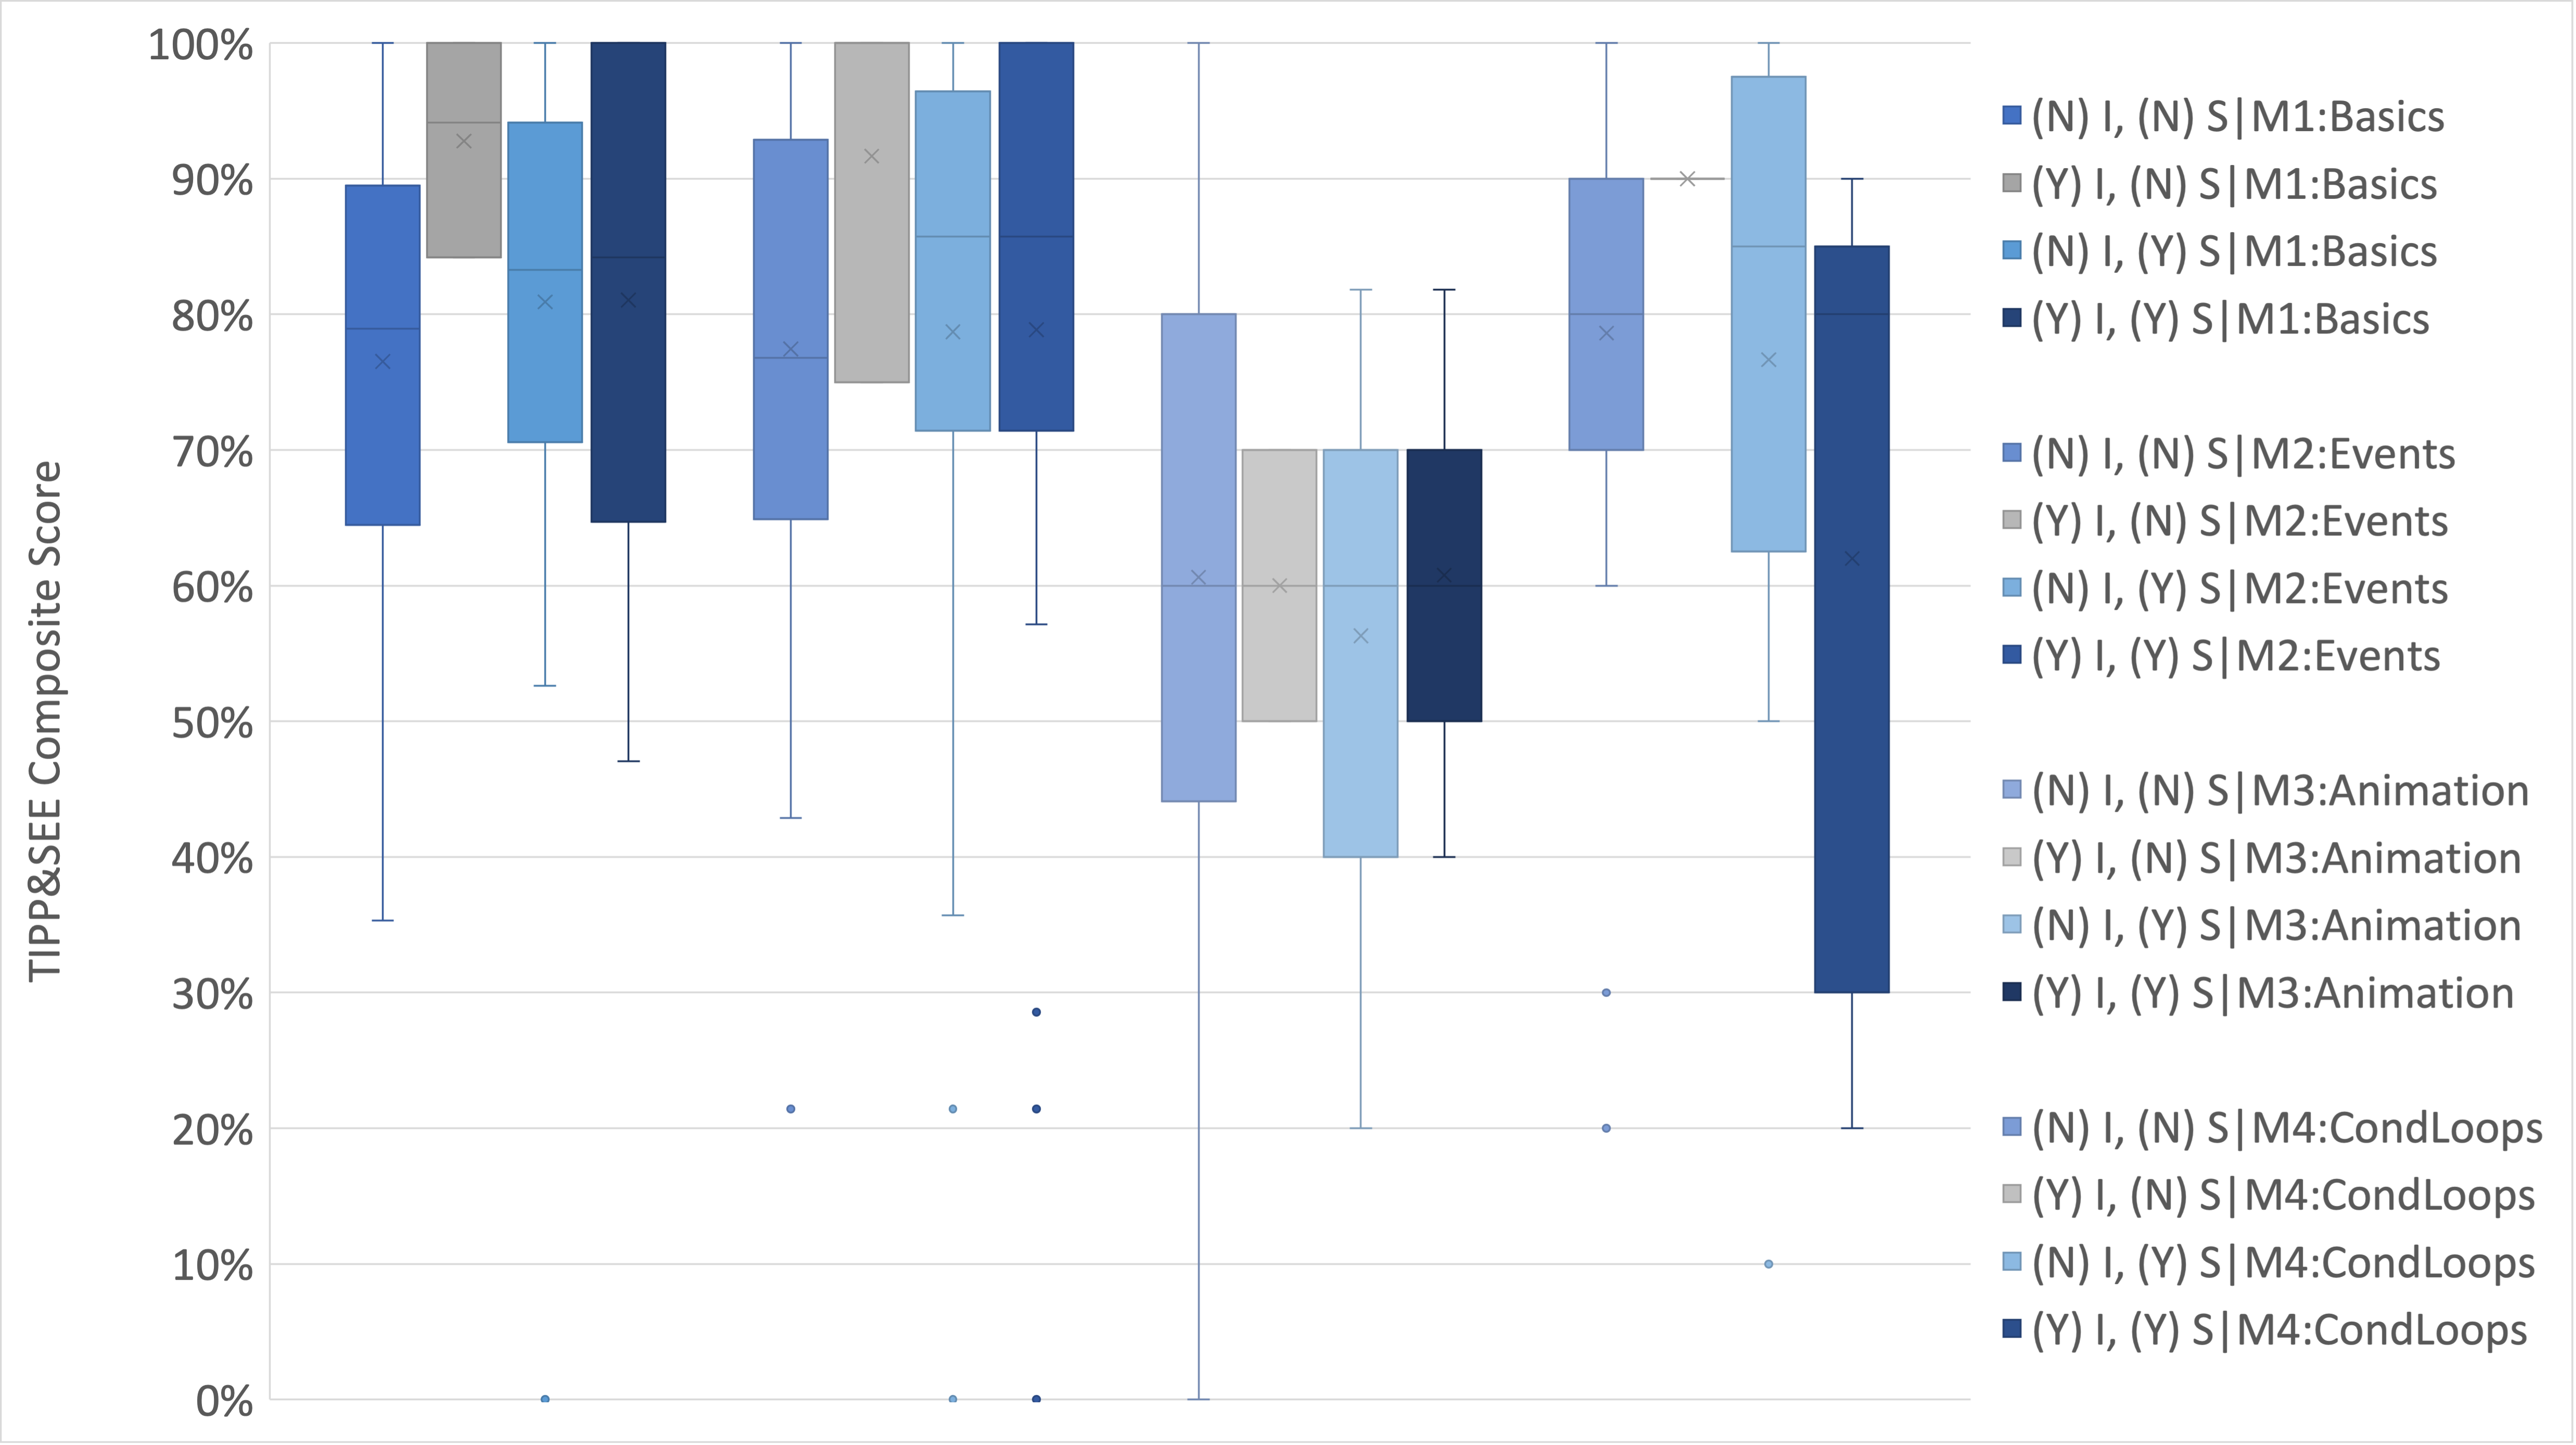
\includegraphics[width=\textwidth]{Previous_Experience.png}}
    \caption{Average \ts Worksheet Composite Scores of Students with Various Combinations of Levels of Informal and In-School Programming Experience} 
    \end{subfigure}
    \caption{\ts Scores Compared Across Levels of Previous STEM Experience}
    \label{fig:math_programming}
\end{figure}

Figure \ref{fig:math_programming} presents: (a) the average composite \ts{} worksheet scores of students whose parents indicated that the student has struggled to complete their mathematics homework in the past compared to those who did not struggle (b) the average composite scores of students stratified by their experience with programming in an informal or school setting. The average \ts{} composite score for students with no mathematics struggle was 91.66\% and the average score for those whose parents reported previous struggles in mathematics coursework was 91.23\%. Our statistical analysis showed that there was no significant difference in performance on \ts{} worksheets between students with and without math struggle in all four modules ($M1: F(2, 147)=1.74, p=.179; M2: F(2,139)=.0552, p=.947; M3: \chi=.366, p=.545; M4: \chi=.00367, p=.952$). As for results based on prior programming experience, the average \ts{} composite score for students with no informal school or programming experience was 91.09\%. For students with informal but no school programming experience, the average was 96.16\%. For those with school but no informal programming experience, the average was 91.99\%. Finally, the average score for those with both school and informal programming experience was 92.09\%. These differences were not statistically significant($M1: \chi=4.32, p=.229; M2: \chi=4.54, p=.209; M3: \chi=.820, p=.845; M4: \chi=3.978, p=.264$). These results are promising and indicate that \ts{} is effective in serving as an equitable learning strategy despite students' struggles in mathematics or previous experiences as reported by their parents.

\subsection{Question-based Factors}
 \label{qb-factors}
 
Lastly, we examined worksheet-based factors. Those factors include the types of questions on the worksheet, whether the questions had a real-world, common-sense, everyday interpretation, and the position of the question within sections of the worksheet. 

\stepcounter{findingnum}
\textit{Finding \arabic{findingnum}: Students attempted "Observe" and "Explore" questions more often than they did "Predict" questions. Students attempted "Observe" questions marginally more than "Explore" questions.}

\begin{figure}
     \centering
     \begin{subfigure}[t]{0.49\textwidth}
        \raisebox{-\height}{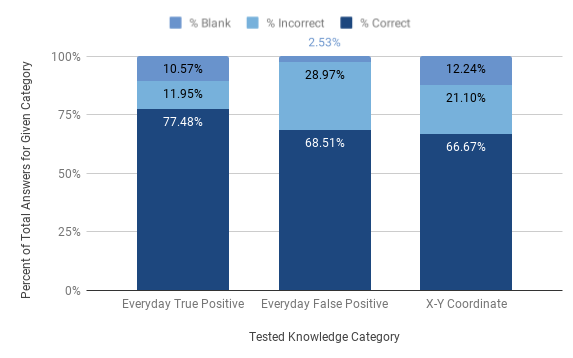
\includegraphics[width=\textwidth]{Observe_Predict_Explore_Overall.png}}
        \caption{Student Performance on 2019-2020 \ts Worksheets by Question Type}
        \label{fig:observe_predict_explore}
    \end{subfigure}
    \hfill
    \begin{subfigure}[t]{0.49\textwidth}
        \raisebox{-\height}{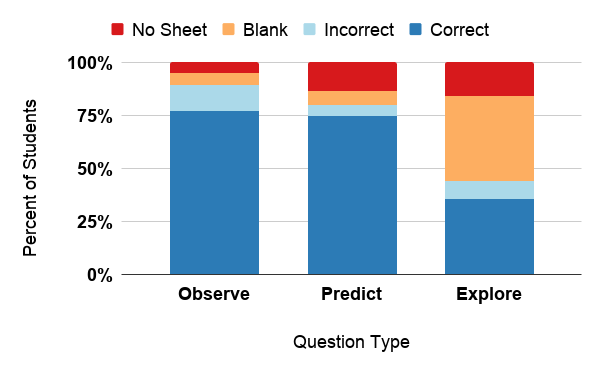
\includegraphics[width=\textwidth]{4Grade_TIPPSEE_Agg_Question.png}}
        \caption{4th Grade Student Performance on \ts Worksheets by Question Type From Previous Study}
        \label{fig:observe_predict_explore_4th}
    \end{subfigure}
    \caption{\ts Scores Compared Across Question Type}
    
\end{figure}

Figure \ref{fig:observe_predict_explore} presents the percent total of correct, incorrect, and blank student answers for each worksheet section: "Observe", "Predict", or "Explore". We found that across modules, students attempted questions within each section of the worksheet at different rates. Students were less likely to attempt and correctly answer “Predict” questions (which asked students to demonstrate a theoretical understanding of the function of blocks) and "Explore questions" (which asked students to make small modifications to existing code to demonstrate a particular concept); the difference was statistically significant ($\chi=71.34, p<.01$). That is, students were least likely to attempt questions that required them to hypothesize about the function of a block or make changes to example code instead of following directions.

Figure \ref{fig:observe_predict_explore_4th} presents findings from previous work on 4th grade students' \ts{} behavior \cite{franklin2020exploring}. While 4th grade students in previous work and the 4th-7th grade students in this study answered "Observe" questions at a similar rate ($\chi=2.86, p=.239$), students in this study were more likely to attempt and correctly answer "Predict" ($\chi=70.86, p<.01$) and "Explore" questions ($\chi=556.43, p<.01$). \hide{They found that across modules, students completed "Observe" and "Predict" questions more and answered them more accurately. A much larger portion of the "Explore" questions were left unanswered.}

\stepcounter{findingnum}
\textit{Finding \arabic{findingnum}: Students were more correct on "Observe" questions than "Predict" and "Explore" questions.} 

Students answered “Predict” and “Explore” questions with comparable correctness, while answering “Observe” questions correctly more than the other two categories. Additionally, "Observe" questions had the fewest incorrect answers while "Explore" questions had the most incorrect answers. As seen in Figure \ref{fig:observe_predict_explore}, "Observe" questions were answered correctly 79.79\% of the time, incorrectly 13.43\% of the time, and left blank 6.78\% of the time. 73.24\% of "Predict" questions were answered correctly, 15.73\% incorrectly, and 11.02\% were left blank. Finally, 73.64\% of "Explore" questions were answered correctly, 18.66\% incorrectly, and 7.70\% were left blank.%say something about these observations holding across the strands that students used or other large-scale observations of students’ attempts. This could be characteristics of questions such as multiple choice/circling etc

\stepcounter{findingnum}
\textit{Finding \arabic{findingnum}: Students are more likely to answer questions and to do so accurately when the block or concept in question has a real-world, common-sense, everyday interpretation.}

Figure \ref{fig:everyday_school} illustrates the differences in answer correctness and answer rate for \ts{} worksheet questions when divided by whether what they were asking students about a concept which matched with its real-world interpretation (Everyday True Positive), did not match with its real-world interpretation (Everyday False Positive), or did not have a straightforward real-world interpretation to begin with and relied primarily on knowledge gained in school settings (School). The figure displays the percent of each response type (correct, incorrect, and blank) in each category. We found a statistically-significant association between response type and the type of knowledge used for a concept ($\chi=55.89, p<.01$). Everyday True Positive questions and Everyday False Positive questions were answered correctly 77.10\% and 80.84\% of the time, respectively, whereas only 68.97\% of School questions were answered correctly. Further, students left 13.13\% of School questions blank, 3.9\% more than Everyday False Positive questions (which were left blank 9.23\% of the time) and 5.46\% more than Everyday True Positive questions (left blank 7.67\% of the time). Additionally, students answered more School questions (17.91\%) incorrectly than Everyday True Positive (15.23\%) and Everyday False Positive (9.93\%) questions.

This data shows that questions testing blocks or concepts that are connected to a school-knowledge meaning are the most likely to be skipped or answered incorrectly by middle grade students when engaging with the \ts{} learning strategy. This behavior may occur because students are associating those blocks or concepts with concepts they have learned in other subjects. Therefore, students who may be less comfortable with certain blocks or concepts, such as variables or blocks that ask students to use the coordinate system.

% this is the "so what" but maybe it belongs in the discussion? I put it both places to decide where it goes better:

%\ts and \scratchencore were created and this study was conducted in order to provide equitable access to intermediate computer science education to middle grade students. In order to do so, it is important to understand if the \ts worksheets impacts student success on theoretical and abstract concepts. In finding 0, we demonstrate that parent-reported previous coursework in programming and mathematics does not impact student engagement or success. In this finding, however, we show that the \ts worksheets that include concepts from previous coursework in mathematics and computer science do impact student engagement as they are the most frequently skipped and the most frequently answered incorrectly. This may be indicative of middle school students' perceptions of the relevance of other coursework to their computer science education. Further research could involve asking students if they perceived the "School" questions as implying that their performance in their other coursework was relevant to their success in their computer science course work. This pre-judgement may cause students to simply not answer the question, if they feel it appears to require knowledge from other coursework.

\stepcounter{findingnum}
\textit{Finding \arabic{findingnum}: The position of a question within a section had an effect on whether or not students were likely to attempt it as well as their correctness.} 

\begin{figure}
     \centering
     \begin{subfigure}{0.49\textwidth}
        \raisebox{-\height}{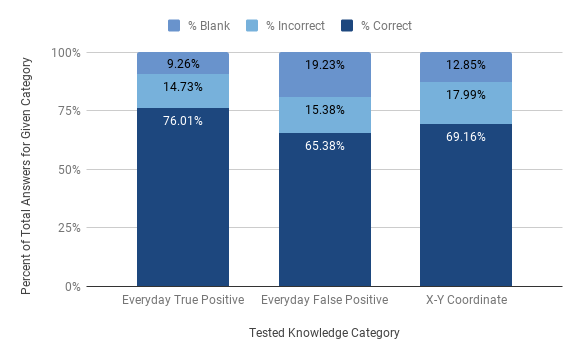
\includegraphics[width=\textwidth]{E_EF_S.png}}
        \caption{Student Performance on 2019-2020 \ts Worksheets by Everyday True Positive, Everyday False Positive, and School-based Knowledge Categorization}
        \label{fig:everyday_school}
    \end{subfigure}
    \begin{subfigure}{0.49\textwidth}
        \raisebox{-\height}{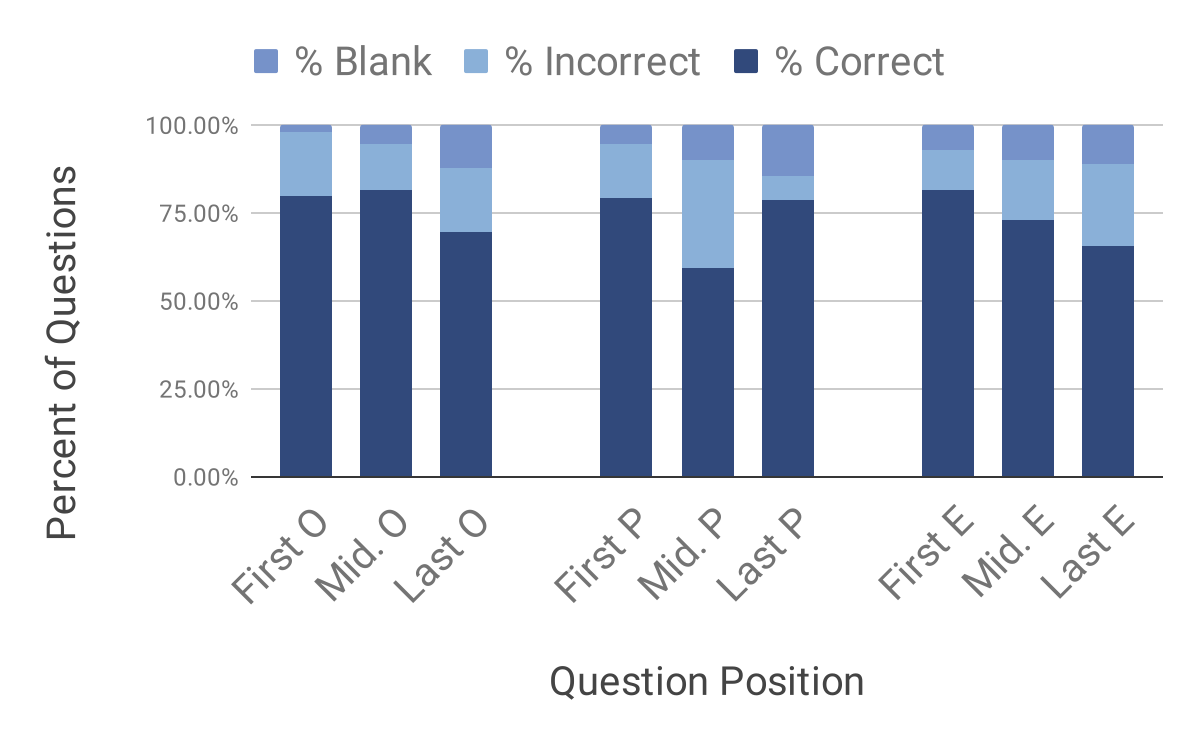
\includegraphics[width=\textwidth]{Position.png}}
        \caption{Average Worksheet Performance by Position in Section on 2019-2020 \ts Worksheets}
        \label{fig:position_es}
    \end{subfigure}
    
    \caption{Student Performance Compared Across Question Position and Question Knowledge-type}
\end{figure}

In Figure ~\ref{fig:position_es}, three lines are shown: correct (percent of attempted questions answered correctly), incorrect (percent of attempted questions answered incorrectly), and blank (percent of questions not attempted) as a function of the position of a question within a section of the worksheet, being the first, middle or last question in a given section. The students tended to attempt fewer questions as they progressed through each section, and the percentage of correct answers decreased through each section ($\chi=76.06, p<.01$). There was similar percentage of incorrect answers from the first to the last question in the sections.

In the "Observe" section there were not any noticeable trends in the percentage of correct or incorrect answers from the first question to the last question. However, there was an increase in blank answers from the first to the last question (first: 5.31\%, middle: 9.81\%, last: 14.50\%). Similarly, we did not observe any noticeable trends in the percentage of correct or incorrect answers in the "Predict" sections. However, there was an increase from 5.31\% to 14.50\% in blank questions for the questions in the "Predict" section.

The position of a question had the strongest impact on answer correctness in the "Explore" section.  For this section, the final section of the worksheets, the percentage of correct answers changed from 81.22\% on the first question to 65.83\% on the last question. In this section, students incorrectly answered twice as many questions at the end of the section as they did at the start of the section (11.64\% to 23.28\%). Additionally, there was an increase in blank answers (first: 7.16\%, middle: 10.00\%, last: 10.94\%).

Despite there being no clear trend in incorrectness/correctness with respect to question position in the individual "Observe" and "Predict" sections, there was an increase in the average percentage of correct answers from the first to last question in all sections. Additionally, the rate of blankness rose steadily from the first to the middle through the last question of all three sections. These findings may be due to the students becoming tired of answering questions from the first to last question in the sections.

\subsection{Correlations between Projects and Worksheets}


